\documentclass[trans,compress,xcolor=pdftex,dvipsnames,table]{beamer}
%\documentclass[compress,xcolor=pdftex,dvipsnames,table]{beamer}

\mode<presentation> {
  \usetheme{CambridgeUS}
  \usecolortheme{rose}
  \usecolortheme{dolphin}
}

\usepackage[english]{babel}
\usepackage[QX]{fontenc}
\usepackage{amssymb}
\usepackage{subfig}
\usepackage[absolute,overlay]{textpos}
\usepackage{colortbl}
\usepackage{multirow}
\usepackage{booktabs}
\usepackage{animate,media9,movie15}
\usepackage[framemethod=TikZ]{mdframed}
\usepackage{bbding}
\usepackage{listings}

\usepackage{tikz}
\usetikzlibrary{calc}

% tikzmark command, for shading over items
\newcommand{\tikzmark}[1]{\tikz[overlay,remember picture] \node (#1) {};}

\newtheorem{algorithm}{Algorithm}

\usepackage{setspace}
\setlength{\TPHorizModule}{1mm}
\setlength{\TPVertModule}{1mm}

\newcommand{\MyLogo}{
\begin{textblock}{14}(109.2,5)
  
\includegraphics[width=1.88cm]{figures/ncmis_logo_small}
 \end{textblock}
}

% user's definition

\newcommand{\minitab}[2][c]{\begin{tabular}{#1}#2\end{tabular}}

\newcommand{\tol}{\mbox{TOL}}
\newcommand{\sK}{\mathcal{K}}
\newcommand{\sN}{\mathcal{N}}
\newcommand{\sC}{\mathcal{C}}
\newcommand{\sF}{\mathcal{F}}
\newcommand{\sG}{\mathcal{G}}
\newcommand{\sT}{\mathcal{T}}
\newcommand{\sA}{\mathcal{A}}
\newcommand{\fA}{\mathfrak A}
\newcommand{\sP}{\mathcal{P}}
\newcommand{\sQ}{\mathcal{Q}}
\newcommand{\sH}{\mathcal{H}}
\newcommand{\sR}{\mathcal{R}}
\newcommand{\sE}{\mathcal{E}}
\newcommand{\sV}{\mathcal{V}}
\newcommand{\dK}{\mathbb{K}}
\newcommand{\dV}{\mathbb{V}}
\newcommand{\trno}[1]{\left|\!\left|\!\left| #1 \right|\!\right|\!\right|}
\newcommand{\tHs}{\tilde{H}^{s}}
\newcommand{\tHns}{H^{-s}}
\newcommand{\ltHs}{H_\Gamma^{s}}
\newcommand{\enorm}[1]{\trno{#1}}
\newcommand{\denorm}[1]{\trno{#1}_*}
\newcommand{\Hsnorm}[1]{\left\|#1\right\|_{\tHs(\Omega)}}
\newcommand{\dHsnorm}[1]{\left\|#1\right\|_{\tHns(\Omega)}}
\newcommand{\dHsw}[1]{\left\| #1 \right\|_{\tHns(\omega_z)}}

\newcommand{\IR}{\mathbb{R}}
\newcommand{\hR}{\widehat R}
\newcommand{\ang}[1]{\left<#1\right>}
\newcommand{\field}{\mathfrak F}
\newcommand{\ubar}{\overline{u}}
\newcommand{\Ubar}{\overline{U}}
\newcommand{\Fbar}{\overline{F}}
\newcommand{\sGbar}{\overline{\sG}}
\newcommand{\ds}{\displaystyle}
\newcommand{\hpsi}{\hat\psi_{\tau}}
\newcommand{\GT}{\left.\overline{\sG_h\psi_z}\right|_{\tau}}
\newcommand{\osc}{\text{\rm osc}}
\newcommand{\Dof}{\text{DOF}}

\newcommand{\bU}{\overline U}
\newcommand{\bu}{\overline u}
\newcommand{\bF}{\overline F}
\newcommand{\sbar}{\overline\Lambda}
\newcommand{\vu}{{\bf{u}}}
\newcommand{\vU}{{\mathbf{U}}}
\newcommand{\vv}{{\bf{v}}}
\newcommand{\vV}{{\mathbf{V}}}
\newcommand{\vF}{{\bf{F}}}
\newcommand{\vf}{{\bf{f}}}
\newcommand{\vg}{{\bf{g}}}
\newcommand{\vh}{{\bf{h}}}
\newcommand{\vI}{{\bf{I}}}
\newcommand{\vC}{{\bf{C}}}
\newcommand{\vX}{{\bf{X}}}
\newcommand{\vL}{{\bf{L}}}
\newcommand{\vW}{{\bf{W}}}
\newcommand{\vH}{{\bf{H}}}
\newcommand{\vR}{{\bf{R}}}

\DeclareMathOperator*{\diag}{diag}

\newcommand{\normV}[1]{\left\|#1\right\|_{\sV}}
\newcommand{\normdualV}[1]{\left\|#1\right\|_{\sV^*}}
\newcommand{\normH}[1]{\left\|#1\right\|_{\sH}}
\newcommand{\starS}{\mathfrak{S}}
\newcommand{\starI}{\mathfrak{I}}


\mdfdefinestyle{mystyle}{leftmargin=0.2cm, rightmargin=0.2cm, linecolor=blue, backgroundcolor=yellow!50, linecolor=blue, linewidth=1pt, roundcorner=5pt}

\mdfdefinestyle{mystyle1}{leftmargin=0.4cm, rightmargin=0.4cm, linecolor=blue, backgroundcolor=yellow!50, linecolor=blue, linewidth=1pt, roundcorner=5pt}

\mdfdefinestyle{mystyle2}{leftmargin=0.05cm, rightmargin=0.05cm, linecolor=blue, backgroundcolor=green!30, linewidth=1pt}

\mdfdefinestyle{mystyle3}{leftmargin=0.4cm, rightmargin=0.4cm, linecolor=red, topline=false, bottomline=false, linewidth=3pt}

\mdfdefinestyle{mystyle4}{leftmargin=0.2cm, linecolor=red, topline=false, bottomline=false, rightline=false, linewidth=4pt}

\setbeamertemplate{footline}{%
  \raisebox{5pt}{\makebox[\paperwidth]{\hfill\makebox[18pt]{\large\color{Blue}\insertframenumber}}}}


% Define the listings environment
\usepackage{listings}
\usepackage{textcomp}
\definecolor{listinggray}{gray}{0.95}
\definecolor{deepblue}{rgb}{0.1,0,0.7}
\definecolor{deepred}{rgb}{0.6,0,0}
\definecolor{deepgreen}{rgb}{0,0.5,0}

\usepackage[utf8]{inputenc}
\DeclareFixedFont{\ttb}{T1}{txtt}{bx}{n}{9} % for bold
\DeclareFixedFont{\ttm}{T1}{txtt}{m}{n}{9} % for normal

\lstset{
        columns=fixed,
        extendedchars=true,
        frame=single,
        linewidth=0.95\linewidth,
        xleftmargin=18pt,
        numbers=left,
        numberstyle=\tiny,
        stepnumber=1,
        backgroundcolor=\color{listinggray},
	tabsize=4,
	language=python,
	basicstyle=\tiny,
	keywordstyle=\color{deepblue},
	emph={MyClass,__init__},          
	emphstyle=\color{deepred},    
	stringstyle=\color{red},
	commentstyle=\color{deepgreen},
	showstringspaces=false,
}

%%% Always I forget this so I created some aliases
\def\ContinueLineNumber{\lstset{firstnumber=last}}
%\def\StartLineAt#1{\lstset{firstnumber=#1}}
%\let\numberLineAt\StartLineAt
  
%%% frame list %%%
\newif\ifframeinlbf
\frameinlbftrue

\makeatletter
\newcommand\listofframes{\vfill\@starttoc{lbf\thesection}}
\makeatother

\addtobeamertemplate{frametitle}{}{%
  \ifframeinlbf
  \addcontentsline{lbf\thesection}{section}{\protect\makebox[2em][l]{%
    \protect\usebeamercolor[fg]{structure}\insertframenumber\hfill}%
  \insertframetitle\vfill}%
  \else\fi%
}

\newif\ifframeinlbf
\frameinlbftrue
\makeatletter
\newcommand\listframes{\@starttoc{lbf}}
\makeatother

\beamertemplatenavigationsymbolsempty

%%%%%%%%%%%%%%%%%%%%%%%%%%%%%%%%%%%%%%%%%%%%
\title[DL Engines]
{\LARGE A Quick Survey on Deep Learning Engines}
%%%%%%%%%%%%%%%%%%%%%%%%%%%%%%%%%%%%%%%%%%%%

\author[Chensong Zhang]{Chensong Zhang}

\institute[LSEC]
{with {\color{RubineRed}Zheng Li} and  {\color{RubineRed}Ronghong Fan}\\[1.5cm]}

\date{\small {\color{OliveGreen}DL Seminar} | {\color{DarkOrchid}April 27, 2017}}

\setbeamercolor{section in toc}{fg=Mahogany}

%%%%%%%%%%%%%%%%%%%%%%%%%%%%%%%%%%%%%%%%%%%%
\begin{document} % Start your content from here ...
%%%%%%%%%%%%%%%%%%%%%%%%%%%%%%%%%%%%%%%%%%%%

\begin{frame}[plain]
  \titlepage
\end{frame}

\addtocounter{framenumber}{-1} % first page does not count

%%%

\frameinlbffalse

\setbeamertemplate{section in toc}{\hspace*{1.2em}\inserttocsection}

{
\usebackgroundtemplate{
\tikz[overlay,remember picture] \node[opacity=0.5, xshift=1.5cm, at=(current page.center)] {

\includegraphics[width=0.7\paperwidth]{figures/deep-learning-brain.png}
};}

\begin{frame}[plain]
  \frametitle{Outline}
  \setcounter{tocdepth}{1}
  {\color{red}\tableofcontents}
\end{frame}
}

\addtocounter{framenumber}{-1} % this page does not count

\frameinlbftrue

%%%

%!TEX root = ../talk.tex

\section{Introduction}\label{sec:intro}

%%%

\frameinlbffalse

{
\usebackgroundtemplate{
\tikz[overlay,remember picture] \node[opacity=0.25, xshift=2.3cm, at=(current page.center)] {
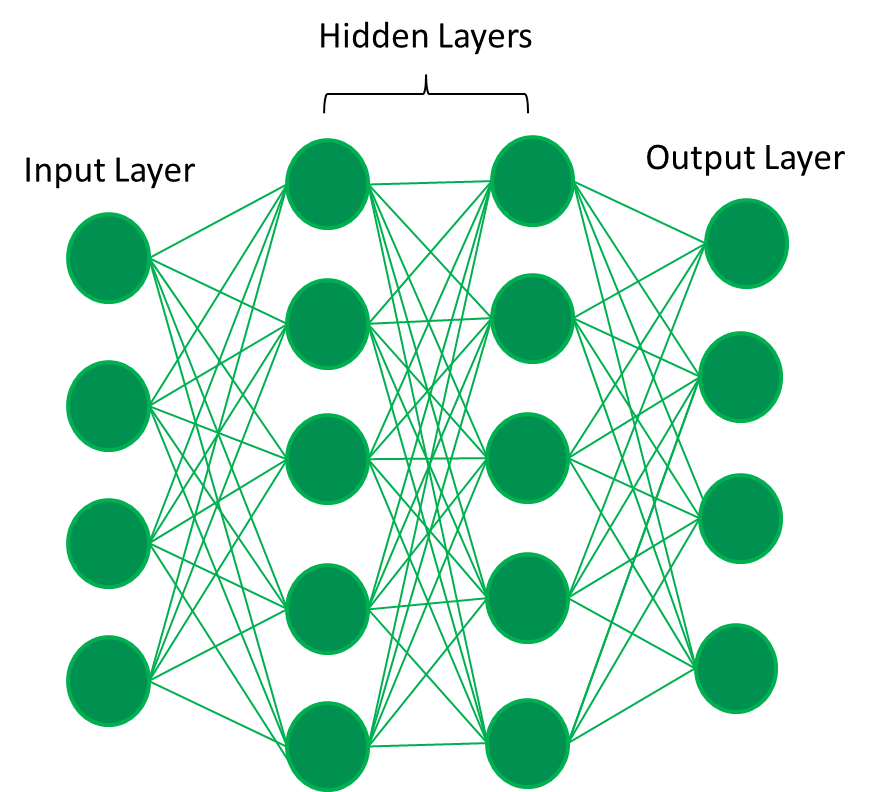
\includegraphics[width=0.65\paperwidth]{figures/genericDNN.png}
};}

\begin{frame}[plain]
\frametitle{\S\ref{sec:intro}. \insertsection}
\listofframes
\end{frame}
\addtocounter{framenumber}{-1} % this page does not count

}

\frameinlbftrue

%%%
\subsection{Background}
%%%

\begin{frame}
  \MyLogo
  \frametitle{Machine Learning}  
\small
\smallskip

\structure{Why ML now?}
\begin{itemize}

\item Unlike traditional numerical simulation, ``ML gives computers the ability to learn without being explicitly programmed'' {\footnotesize\color{DarkOrchid}[Samuel 1959]}

\item As a research field, ML explores the study and construction of algorithms that can \alert{learn} from and \alert{make predictions} on \alert{data}

\item Fourth paradigm, big data, artificial intelligence, Internet of things, ...

\end{itemize}

\structure{General Tasks of ML:}

\begin{itemize}

\item Classification: Inputs are divided into two or more classes, and the learner must produce a model that assigns unseen inputs to one or more (multi-label classification) of these classes

\item Clustering: Inputs are divided into groups. Unlike in classification, the groups are not known beforehand, making this typically an unsupervised task

\item Regression: Similar to classification, but the outputs are continuous

\item Density estimation, dimensionality reduction, ...

\end{itemize}

\begin{center}
{\color{red} \scriptsize
I. Goodfellow, Y. Bengio, and A. Courville,
https://github.com/exacity/deeplearningbook-chinese
}
\end{center}
\end{frame}

%%%

\begin{frame}
  \MyLogo
  \frametitle{Software Packages for Machine Learning}  
\small

\structure{What is the purpose?}
\begin{itemize}
\item Solving problems from practical applications (user interface)
\item Developing algorithms and optimizing implementation (development)
\item Theoretical analysis for machine learning
\end{itemize}

\structure{What do we want for a ML package?}
\begin{itemize}
\item Easy for new tasks and new network structures (less steep learning curve)
\item Easy for debugging (with good support and large community)
\item Performance and scalability
\end{itemize}

\vskip -12pt
\begin{figure}[htbp] %  figure placement: here, top, bottom, or page
   \centering
   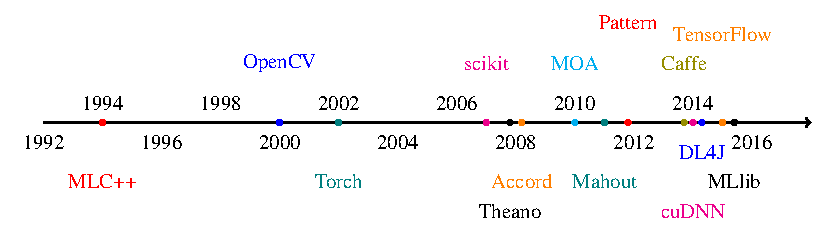
\includegraphics[width=0.9\linewidth]{figures/ML.pdf} 
\end{figure}

\begin{center}
{\color{red} \scriptsize
Tour of TensorFlow, by Peter Goldsborough, arXiv, 2016}
\end{center}


\end{frame}

%%%
\subsection{DL code}
%%%

\begin{frame}
  \MyLogo
  \frametitle{Deep Learning: Pros and Cons}  

\small

\begin{mdframed}[style=mystyle2]
Deep Learning has been introduced with the objective of moving ML closer to one of its original goals---AI. The main motivations includes:
%
\begin{itemize}\scriptsize\setlength\itemsep{0.2em}
\item Insufficient depth can hurt
\item The brain has a deep architecture
\item Cognitive processes seem deep
\end{itemize}
\end{mdframed}

\medskip

\begin{columns}

\column{.49\textwidth}
{\color{blue}Pros:}
\begin{itemize}\setlength\itemsep{0.2em}
\item conceptually simple
\item nonlinear 
\item highly flexible and configurable
\item learned features can be extracted
\item can be fine-tuned with more data
\item efficient for multi-class problems
\item world-class at pattern recognition
\end{itemize}

\column{.51\textwidth}
{\color{red}Cons:}
\begin{itemize}\setlength\itemsep{0.2em}
\item hard to interpret 
\item theory not well understood
\item slow to train and score
\item overfits, needs regularization
\item more parameters
\item inefficient for categorical variables
\item data hungry, learns slowly 
\end{itemize}
\end{columns}

\begin{center}
{\color{red} \scriptsize
https://www.slideshare.net/0xdata/transform-your-business-with-ai-deep-learning-and-machine-learning}
\end{center}

\end{frame}

%%%
\subsection{General comparison}
%%%

\begin{frame}
  \MyLogo
  \frametitle{Popular Packages: Basic Information}  
\small

\renewcommand{\multirowsetup}{\centering} 
\begin{table}[htdp]
\begin{center}
\begin{tabular}{|c|c|c|c|c|c|} \hline
\rowcolor{GreenYellow}
Viewpoint &Torch       &Caffe   & TensorFlow  & MXNet \\ \hline
Released      & 2002      &2013               &2015                & 2015                    \\ \hline
 \multirow{3}{4em}{Main \\ Developers}
 & Facebook,        &\multirow{3}{5em}{BAIR \\ BVLC}  &\multirow{3}{3em}{Google} &\multirow{3}{*}{DMLC}   \\ 
 &Twitter,            & & &    \\
 &Google, ...       & & &  \\ \hline 
\multirow{2}{4em}{ Core \\ Languages}     
& \multirow{2}{3em}{ C/Lua }      
&\multirow{2}{4em}{ C++}
&\multirow{2}{4em}{ C++\\Python}
&\multirow{2}{6em}{ C++}  \\ 
&   &    & &      \\ \hline
\multirow{2}{4em} {Supported \\Interface }    
& \multirow{2}{3em}{ Lua }      
&\multirow{2}{5.5em}{ C++/Python \\ Matlab}
&\multirow{2}{5.5em}{ C++/\alert{Python} \\ \alert{R}/Java/Go}  
&\multirow{2}{5.5em}{ C++/\alert{Python} \\ \alert{R}/Julia/Matlab}\\  
&   &    & &      \\ \hline           
 \multirow{2}{4em}{ License }     
& \multirow{2}{3em}{BSD}      
&\multirow{2}{4em}{BSD}
&\multirow{2}{4em}{Apache}
&\multirow{2}{6em}{Apache}  \\ 
&   &    & &      \\ \hline
\end{tabular}
\end{center}
\label{default}
\end{table}%

\vskip -10pt
{\scriptsize
\begin{itemize}\setlength\itemsep{0.5em}
\item[\raisebox{-0.4ex}{\alert{\HandRight}}] Other worth-noting's: CNTK/DMTK (Microsoft), Neon (Nervana \& Intel), PyTorch (\alert{beta})
\item BAIR, Berkeley Artificial Intelligence Research Lab 
\item BVLC, Berkeley Vision and Learning Center
\item DMLC, Distributed (Deep) Machine Learning Community, supported by Amazon, Intel, Microsoft, nVidia, Baidu, ...
\end{itemize}
}

\begin{center}
{\color{red}\scriptsize
http://blog.revolutionanalytics.com/2016/08/deep-learning-part-1.html
}
\end{center}

\end{frame}

%%%

\begin{frame}
  \MyLogo
  \frametitle{Popular Packages: Performance}  
\small

\renewcommand{\multirowsetup}{\centering} 
\begin{table}[htdp]
\begin{center}
\begin{tabular}{|c|c|c|c|c|c|} \hline
\rowcolor{GreenYellow}
Viewpoint &Torch       &Caffe  & TensorFlow & MXNet  \\ \hline
  \multirow{2}{4em}{Pretrained \\ Models}      
  &  \multirow{2}{4em} {Yes}      
  &  \multirow{2}{4em}{Yes}                             
  &  \multirow{2}{4em}{No}                   
  &  \multirow{2}{4em}{Yes}\\ 
  &  &   &   & \\ \hline
\multirow{2}{4.5em}{High-level \\ Support}     
& \multirow{2}{*}{Good}      
&\multirow{2}{*}{ Good}
&\multirow{2}{*}{ Good}
&\multirow{2}{*}{ Good}  \\ 
&   &    & &      \\ \hline
 \multirow{2}{4em}{Low-level \\ Operators}
 &\multirow{2}{4em}{Good}
 &\multirow{2}{*}{Good }     
 &\multirow{2}{*}{Fairly good}
 &\multirow{2}{*}{Very few}\\ 
 &       &    &  &  \\ \hline 
\multirow{2}{4em} {Speed \\ One-GPU }    
& \multirow{2}{*}{ Great }      
&\multirow{2}{*}{Great} 
&\multirow{2}{*}{\alert{Not so good}}
&\multirow{2}{*}{ Excellent} \\  
&   &    & &      \\ \hline          
\multirow{2}{5em} {Memory \\ Management}    
& \multirow{2}{*}{ Great }      
&\multirow{2}{*}{Great}
&\multirow{2}{*}{\alert{Not so good}}
&\multirow{2}{*}{ Excellent}  \\  
&   &    & &      \\ \hline            
\multirow{2}{3.5em} {Parallel \\ Support}    
& \multirow{2}{5.em}{Multi-GPU}      
&\multirow{2}{5.em}{Multi-GPU}
&\multirow{2}{5.em}{Multi-GPU} 
&\multirow{2}{5em}{Distributed} \\  
&   &    & &      \\ \hline            
\multirow{2}{3.5em} {Coding \\ Style}    
& \multirow{2}{5.em}{Imperative}      
&\multirow{2}{5.em}{Imperative}
&\multirow{2}{5.em}{Declarative} 
&\multirow{2}{5em}{Declarative \\ Imperative} \\  
&   &    & &      \\ \hline
\multirow{2}{3.5em} {GitHub \\ Watching}    
& \multirow{2}{5.em}{649/268}      
&\multirow{2}{5.em}{1856}
&\multirow{2}{5.em}{4939} 
&\multirow{2}{5em}{887} \\  
&   &    & &      \\ \hline
\end{tabular}
\end{center}
\label{default}
\end{table}%

\end{frame}

%!TEX root = ../talk.tex

\section{Comparison}\label{sec:numer}

%%%

\frameinlbffalse

{
\usebackgroundtemplate{
\tikz[overlay,remember picture] \node[opacity=0.4, at=(current page.center)] {
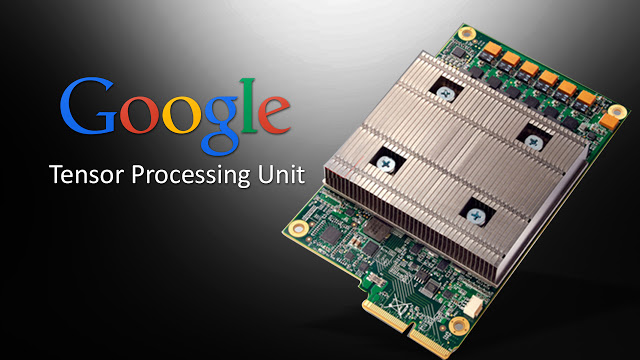
\includegraphics[width=1.15\paperwidth,height=0.68\paperwidth]{figures/tpu.jpg}
};}

\begin{frame}[plain]
\frametitle{\S\ref{sec:numer}. \insertsection}
\listofframes
\end{frame}
\addtocounter{framenumber}{-1} % this page does not count

}

\frameinlbftrue

%%%
\subsection{CPU tests}
%%%

\begin{frame}
	\MyLogo
	\frametitle{CPU Scalability: FCN Synthetic}  

\begin{figure}[htbp] 
	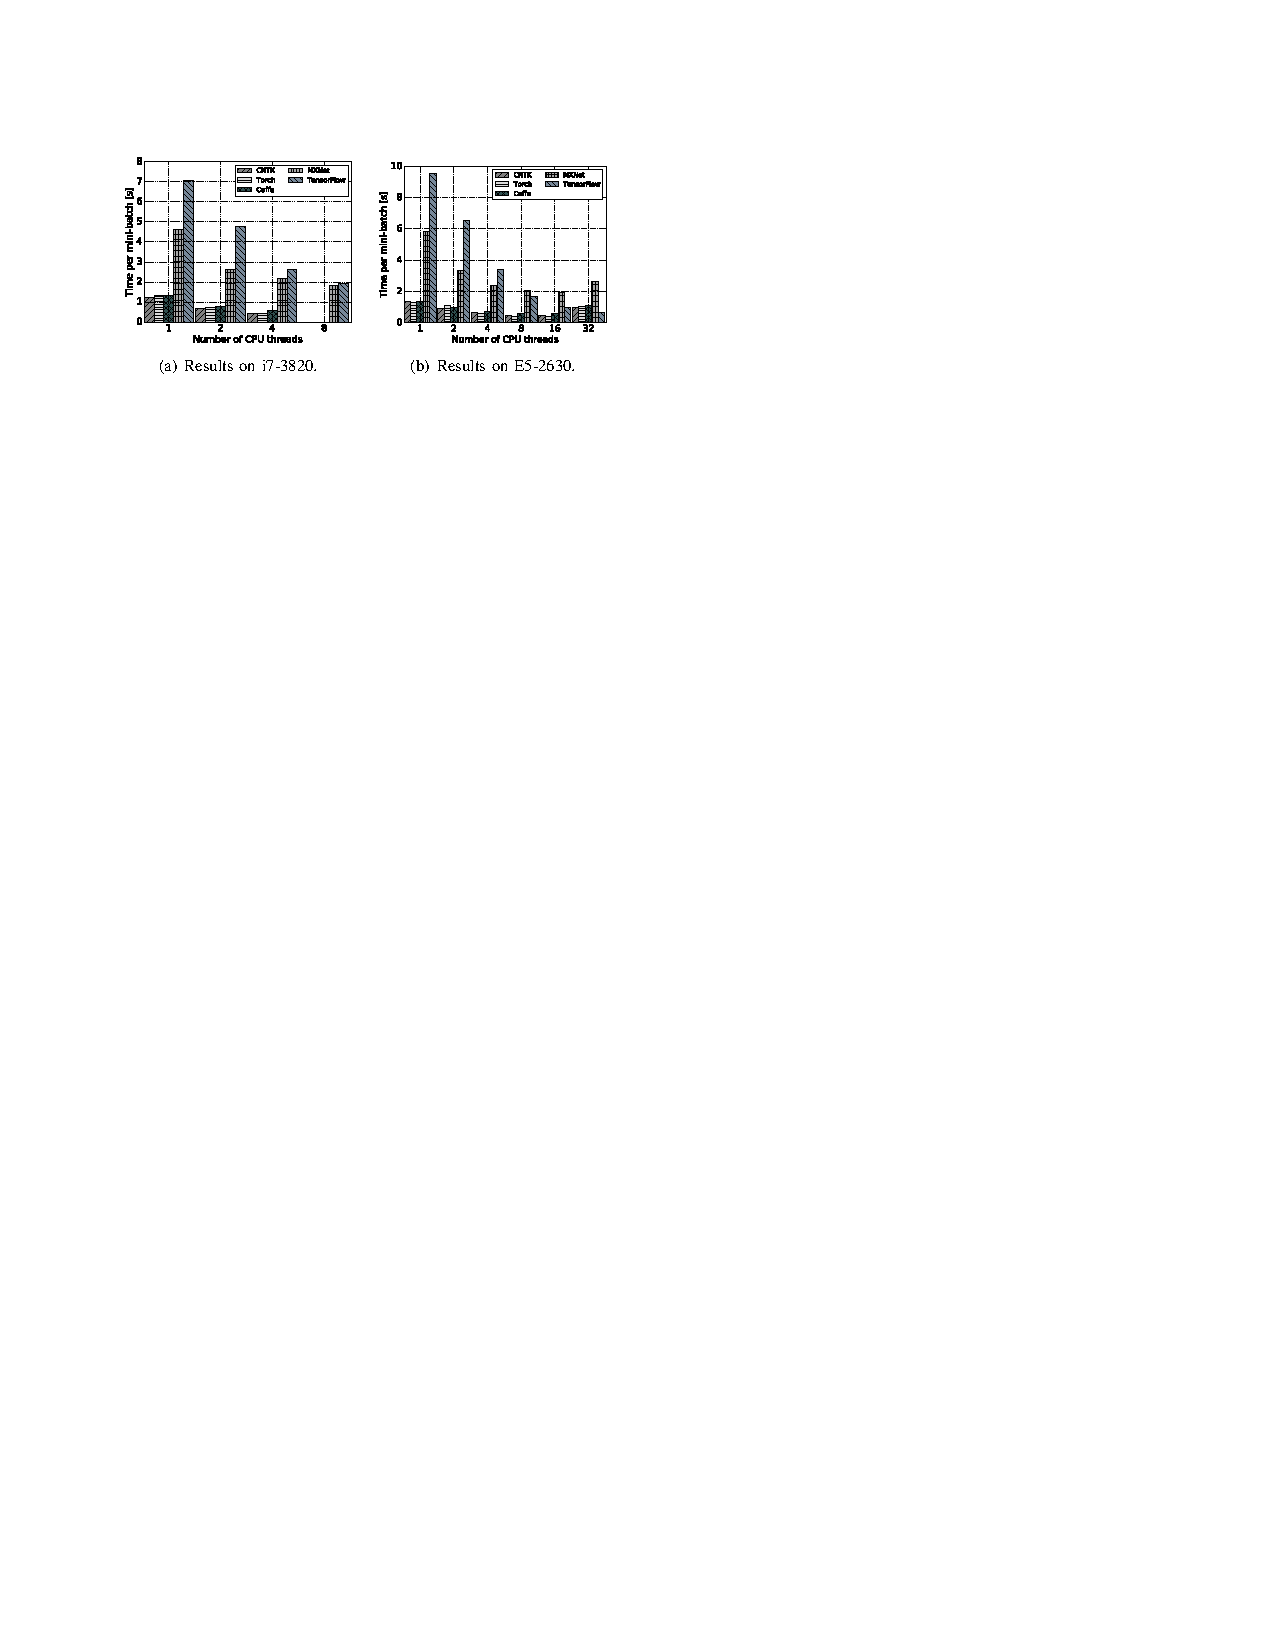
\includegraphics[width=\linewidth]{figures/FCN-S1.pdf} 
	\caption{FCN-S performance on CPU platform with a mini-batch size of 64}
\end{figure}
	
\vskip -10pt
\begin{mdframed}[style=mystyle1]
\begin{itemize}
\item CNTK/Torch/Caffe have similar CPU performance
\item TensorFlow has excellent scalability
\end{itemize}
\end{mdframed}

\end{frame}

%%%

\begin{frame}
	\MyLogo
	\frametitle{CPU Scalability: FCN Real}  
	\begin{figure}[htbp] 
		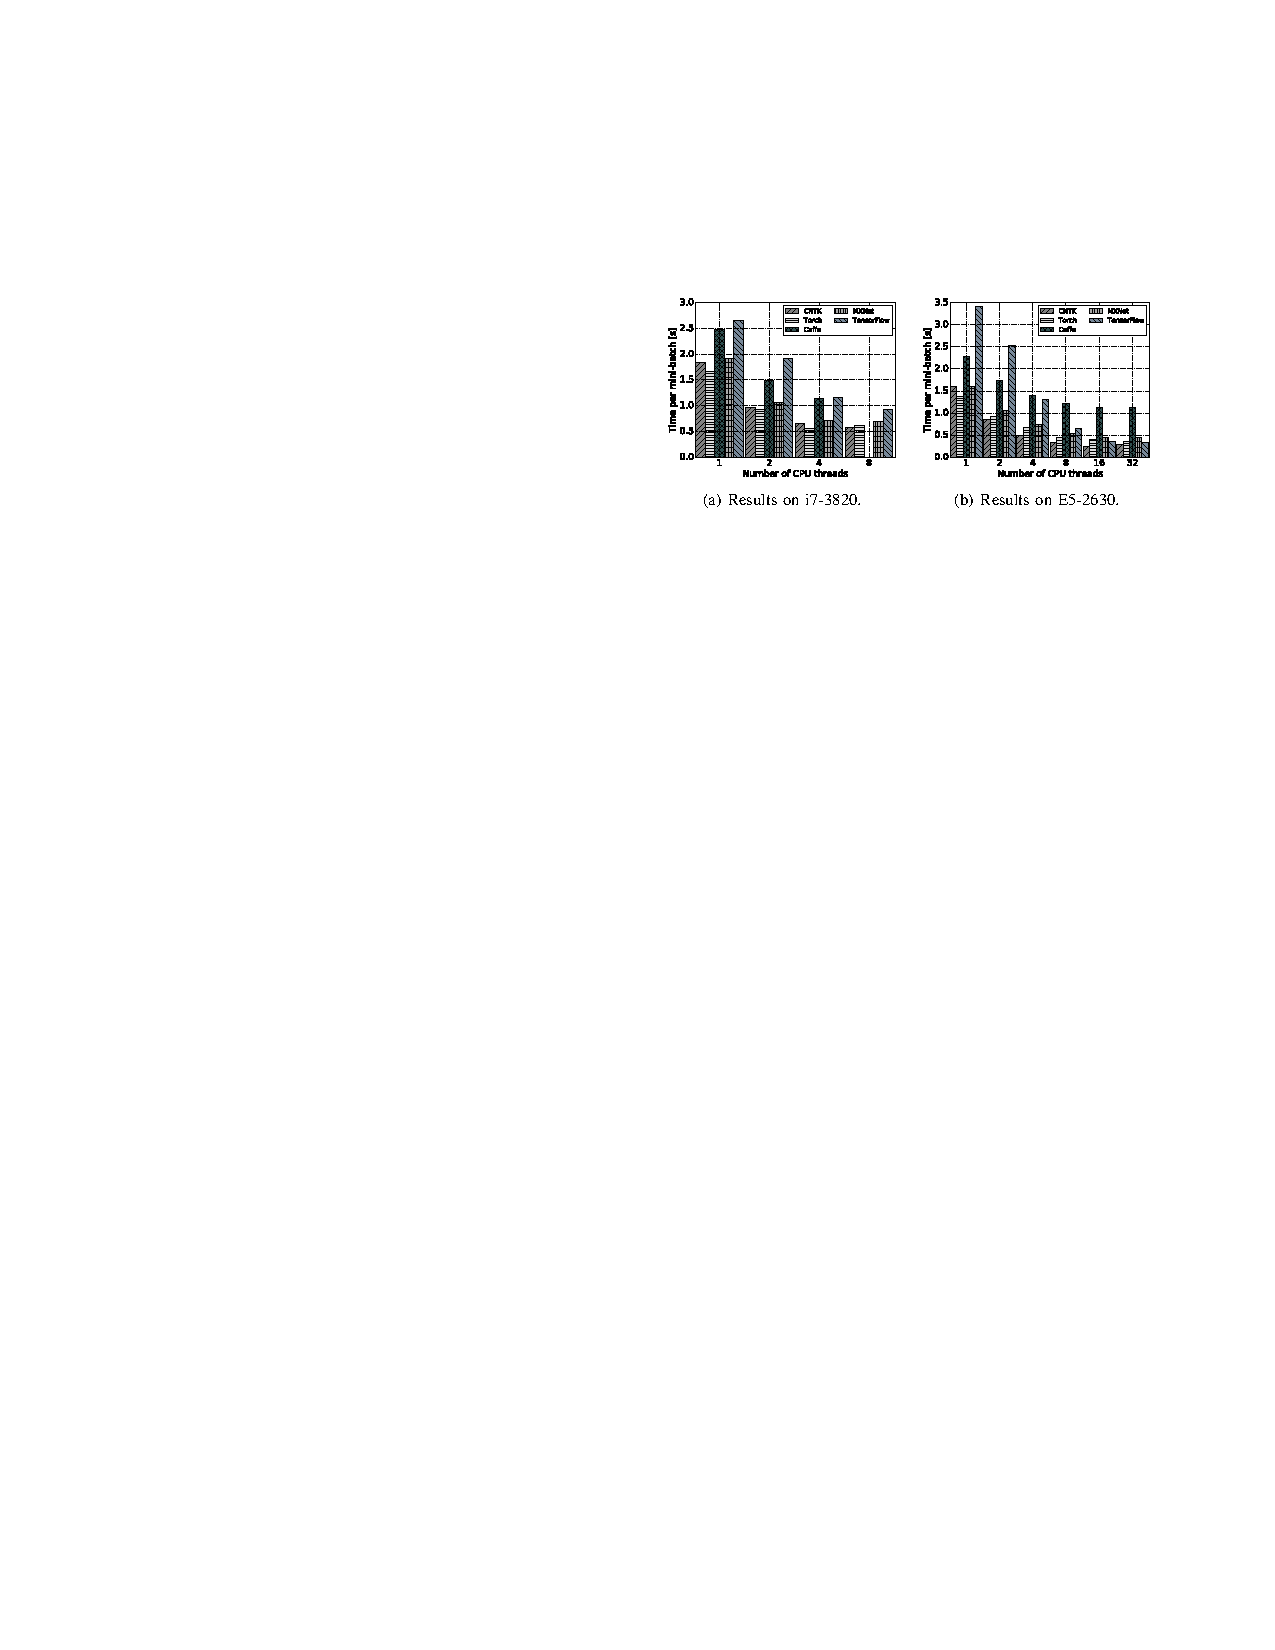
\includegraphics[width=\linewidth]{figures/FCN-R1.pdf} 
		\caption{The FCN-R performance on CPU platform with a mini-batch size of 1024}
	\end{figure}
	
\vskip -10pt
\begin{mdframed}[style=mystyle1]
\begin{itemize}
\item All engines have good CPU performance
\item TensorFlow has good scalability but considerably slower
\end{itemize}
\end{mdframed}

\end{frame}

%%%

\begin{frame}
	\MyLogo
	\frametitle{CPU Scalability: CNN Synthetic}  

	\begin{figure}[htbp] 
		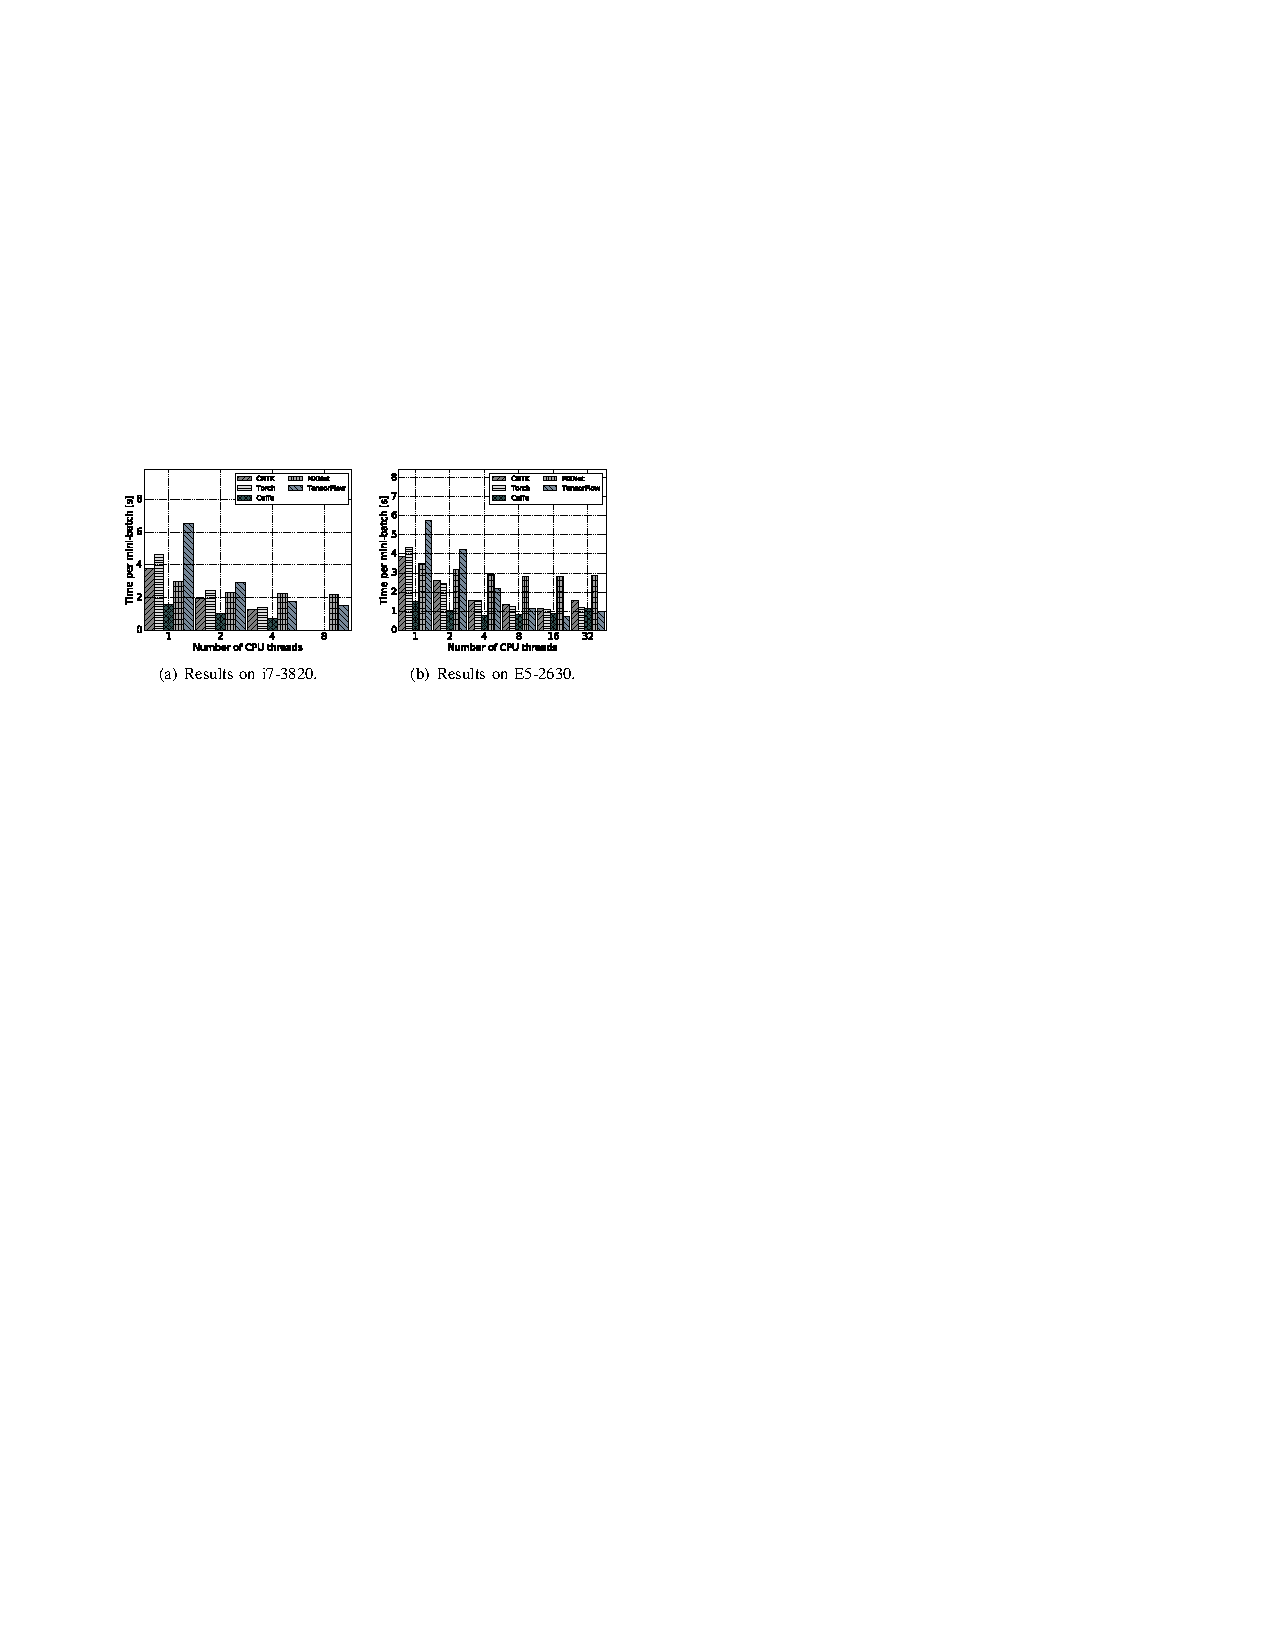
\includegraphics[width=\linewidth]{figures/AlexNet-S1.pdf} 
		\caption{AlexNet-S performance on CPU platform with a mini-batch size of 16}
	\end{figure}
	
\vskip -10pt
\begin{mdframed}[style=mystyle1]
\begin{itemize}
\item Caffe has best CNN performance as promised
\item MXNet does not scale well for this test
\end{itemize}
\end{mdframed}
	
\end{frame}

%%%

\begin{frame}
	\MyLogo
	\frametitle{CPU Scalability: CNN Real}  
	\begin{figure}[htbp] 
		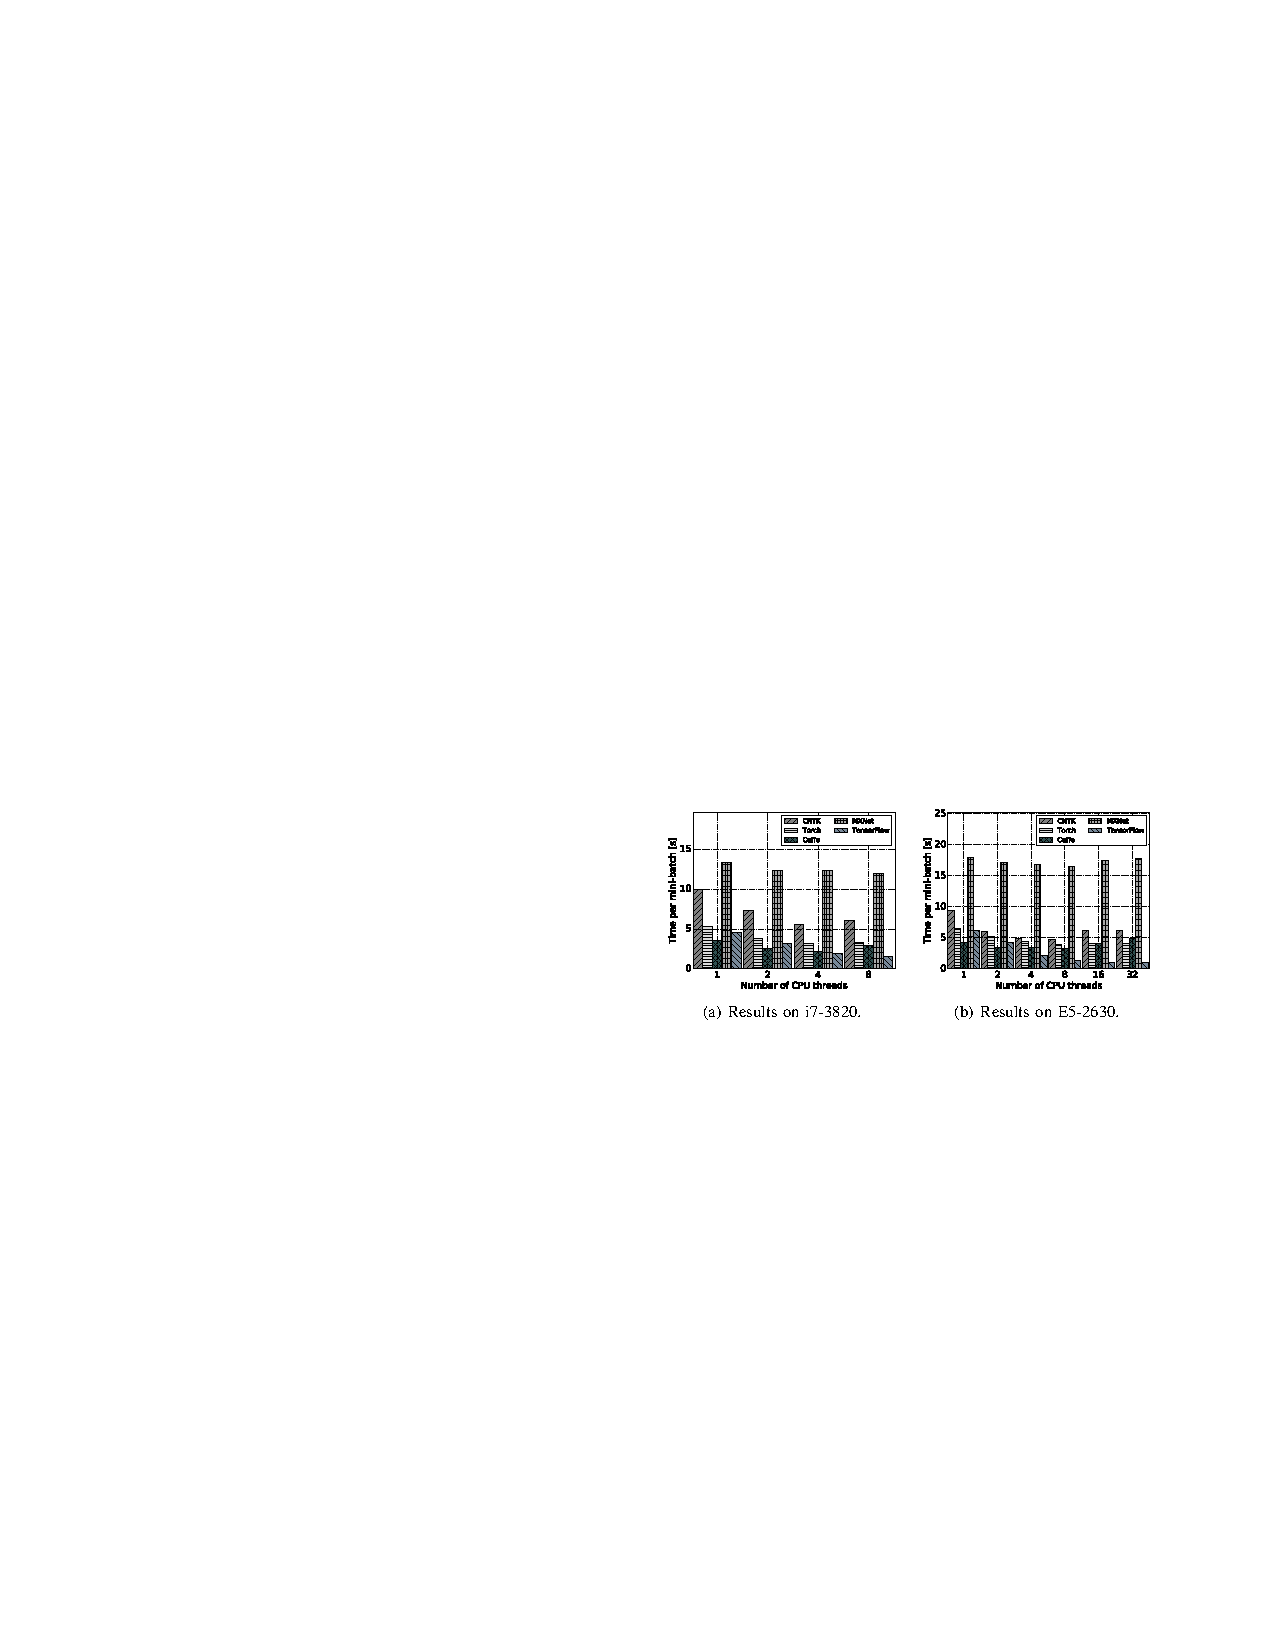
\includegraphics[width=\linewidth]{figures/AlexNet-R1.pdf} 
		\caption{AlexNet-R performance on CPU platform with a mini-batch size of 1024}
	\end{figure}
	
\vskip -10pt
\begin{mdframed}[style=mystyle1]
\begin{itemize}
\item Good scalability of TensorFlow kicks in 
\item Caffe does not scale well on multicore CPUs
\end{itemize}
\end{mdframed}

\end{frame}

%%%

\begin{frame}
	\MyLogo
	\frametitle{CPU Scalability: RNN LSTM}  
	\begin{figure}[htbp] 
		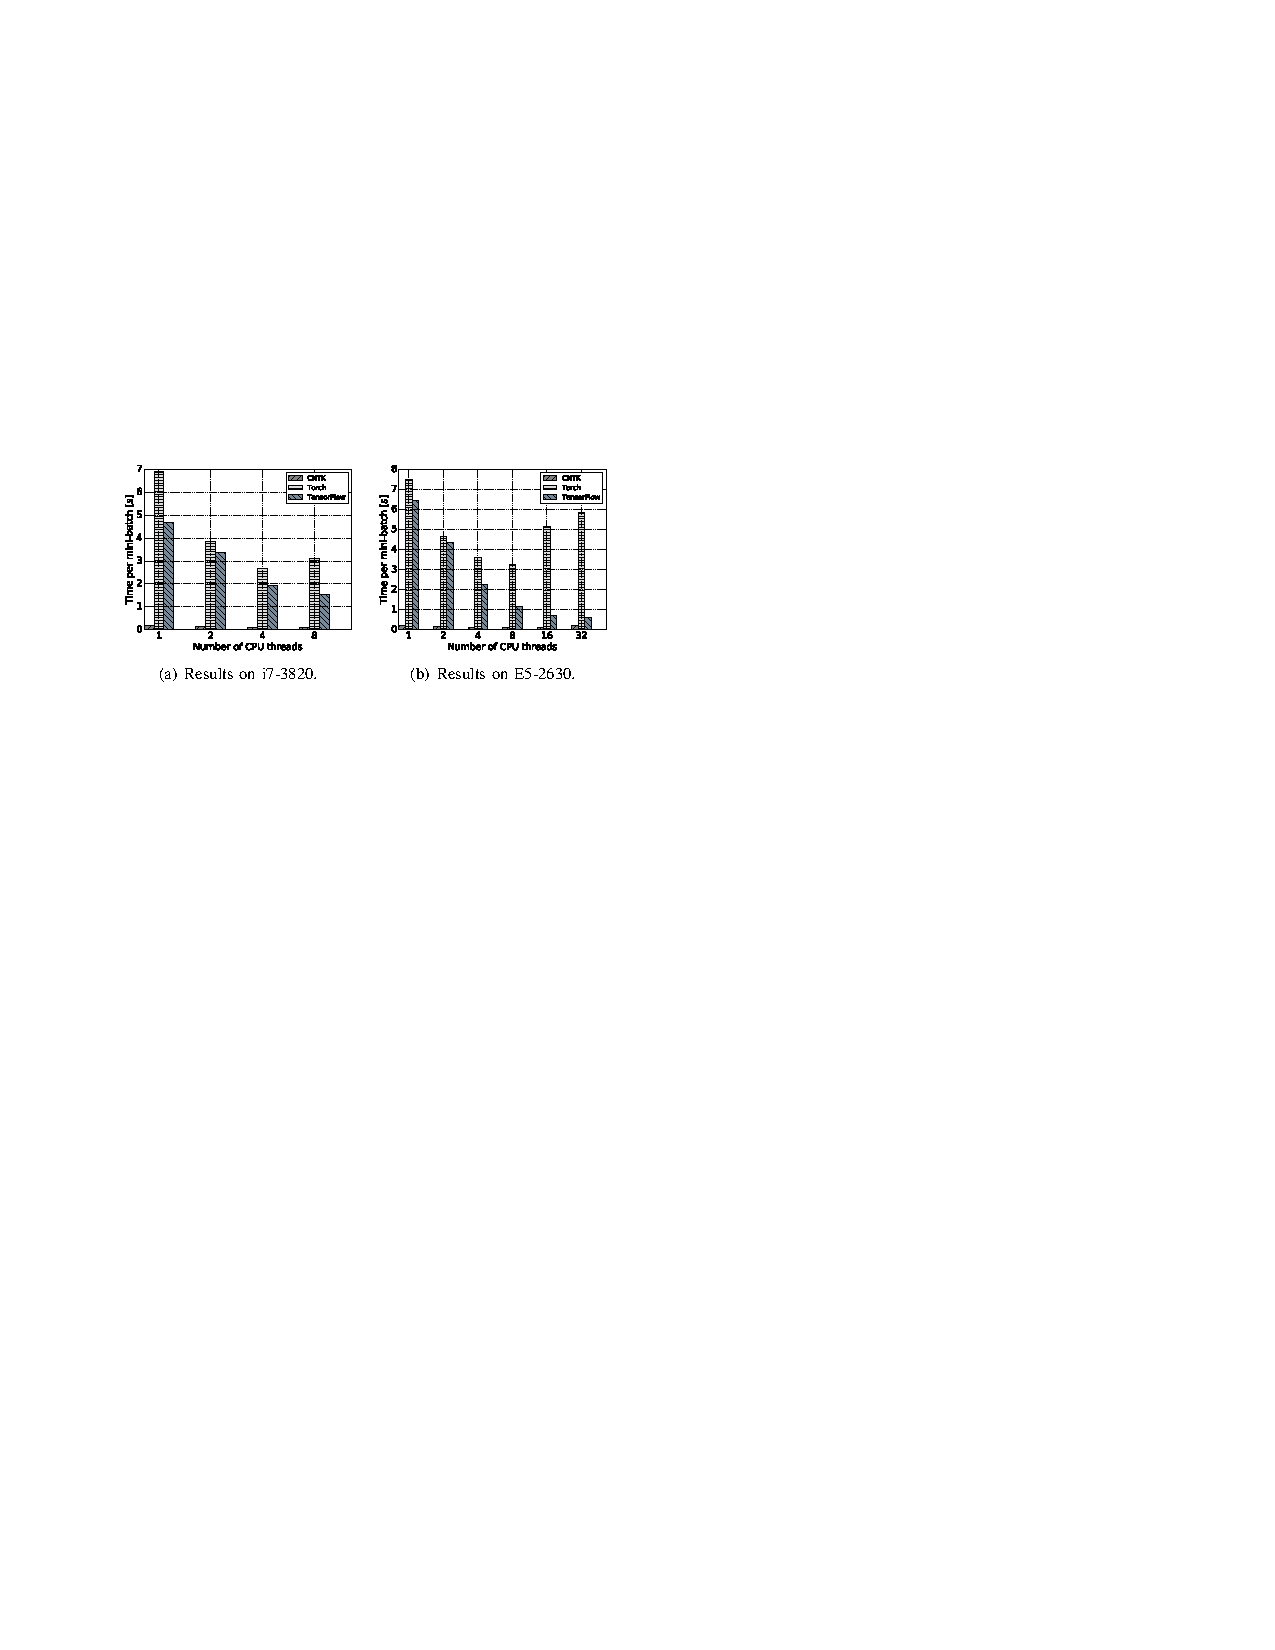
\includegraphics[width=\linewidth]{figures/LSTM1.pdf} 
		\caption{LSTM performance on CPU platform with a mini-batch size of 256}
	\end{figure}
	
\vskip -10pt
\begin{mdframed}[style=mystyle1]
\begin{itemize}
\item Pay more attention to CNTK in the future
\item Caffe/MXNet does not support LSTM on CPUs
\end{itemize}
\end{mdframed}

\end{frame}

%%%
\subsection{GPU tests}
%%%

\begin{frame}
	\MyLogo
	\frametitle{GPU Scalability: FCN Synthetic}

	\begin{figure}[htbp] 
		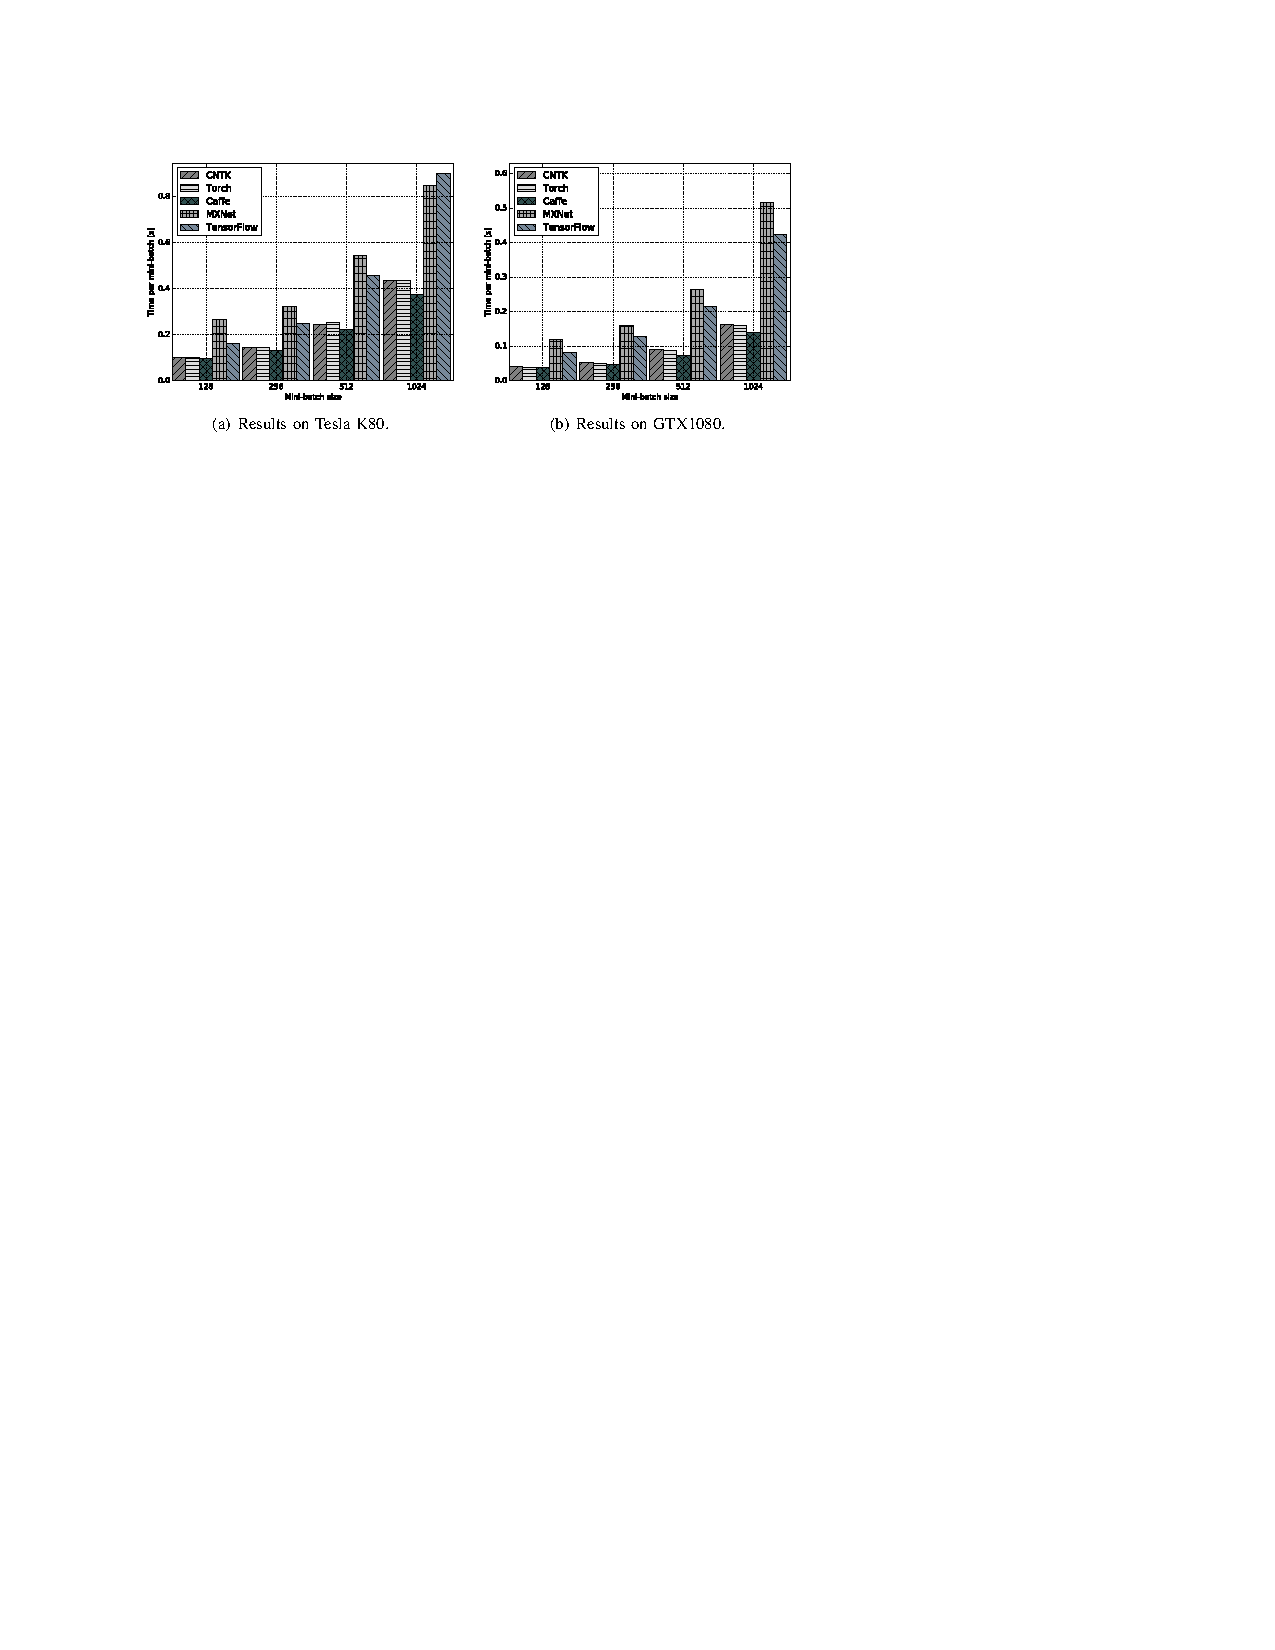
\includegraphics[width=\linewidth]{figures/FCN-S2.pdf} 
		\caption{The performance comparison of FCN-S on GPU platforms}
	\end{figure}

\vskip -10pt
\begin{mdframed}[style=mystyle1]
\begin{itemize}
\item CNTK/Torch/Caffe out-perform the others
\end{itemize}
\end{mdframed}

\end{frame}

%%%

\begin{frame}
	\MyLogo
	\frametitle{GPU Scalability: FCN Real}
	
	\begin{figure}[htbp] 
		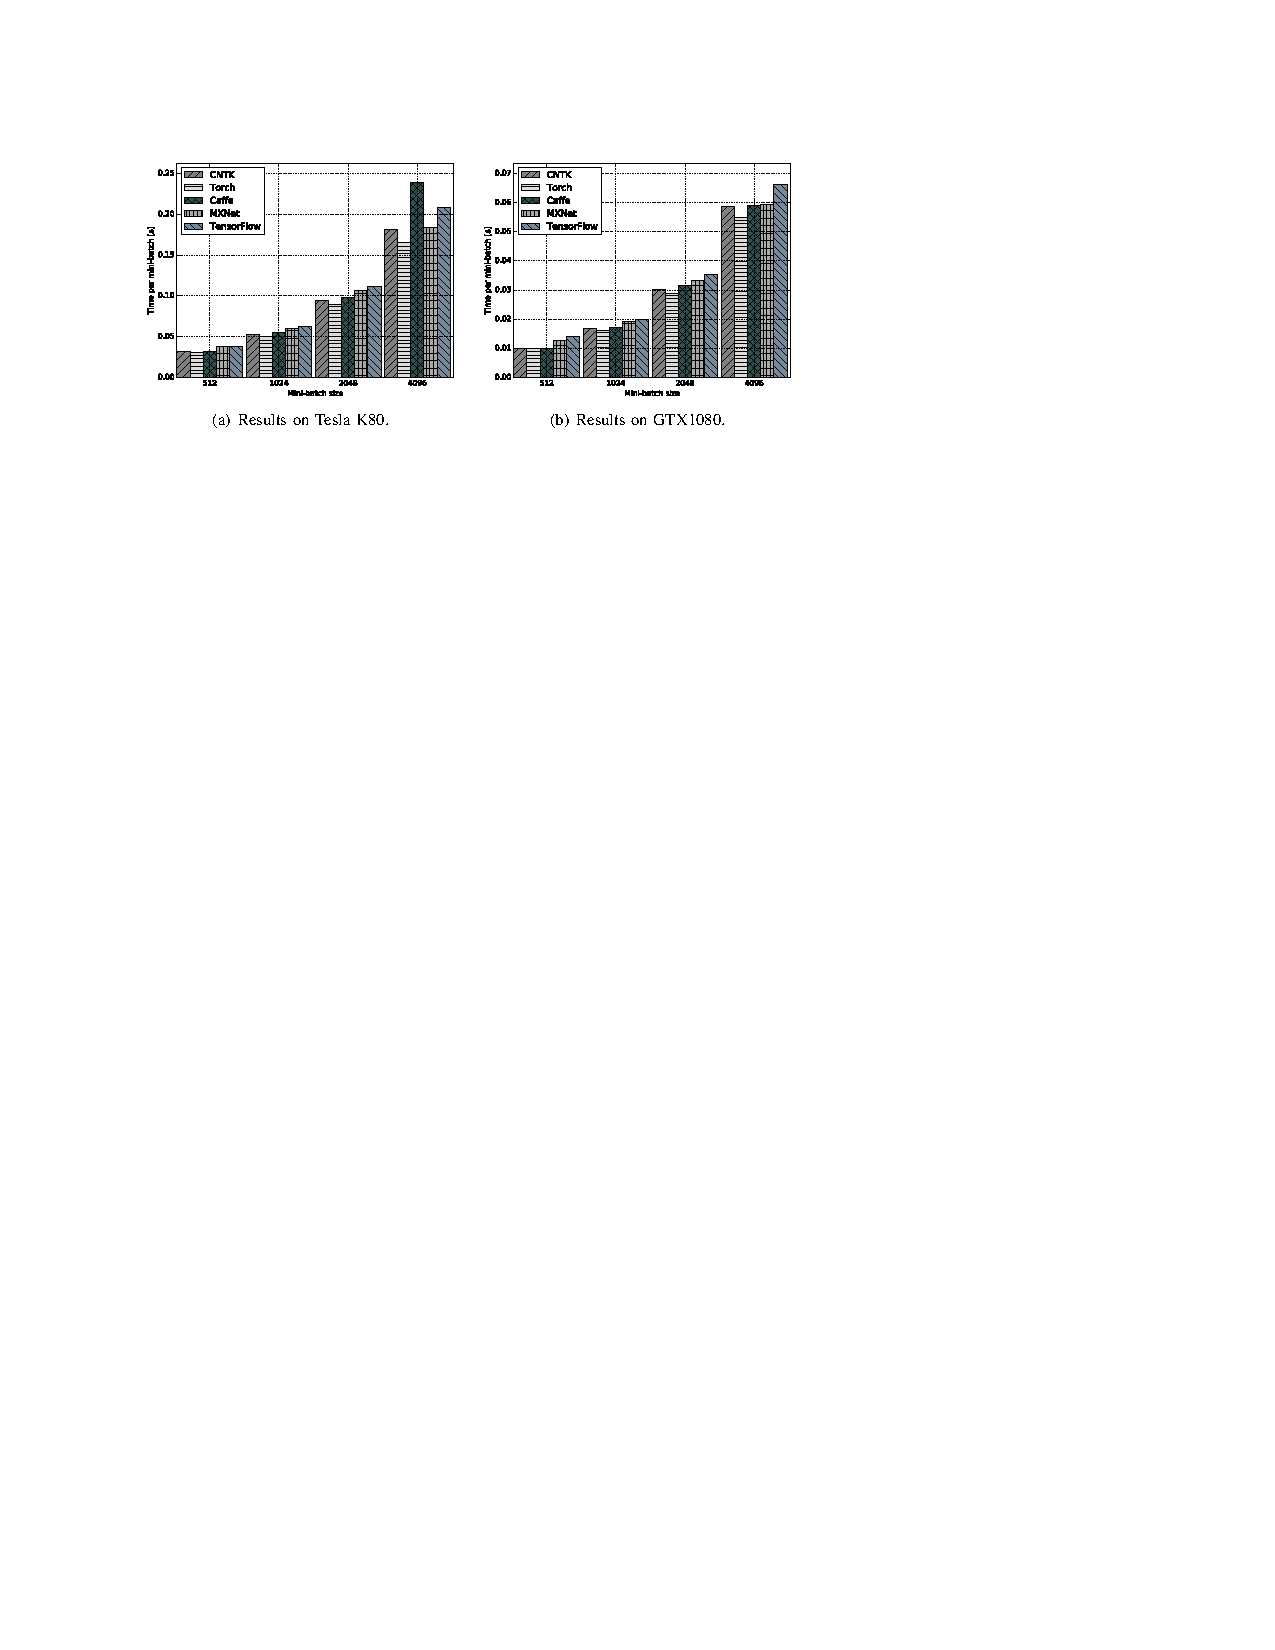
\includegraphics[width=\linewidth]{figures/FCN-R2.pdf} 
		\caption{The performance comparison of FCN-R on GPU platforms}
	\end{figure}

\vskip -10pt
\begin{mdframed}[style=mystyle1]
\begin{itemize}
\item All packages have similar performance
\end{itemize}
\end{mdframed}

\end{frame}

%%%

\begin{frame}
	\MyLogo
	\frametitle{GPU Scalability: CNN Synthetic}

	\begin{figure}[htbp] 
		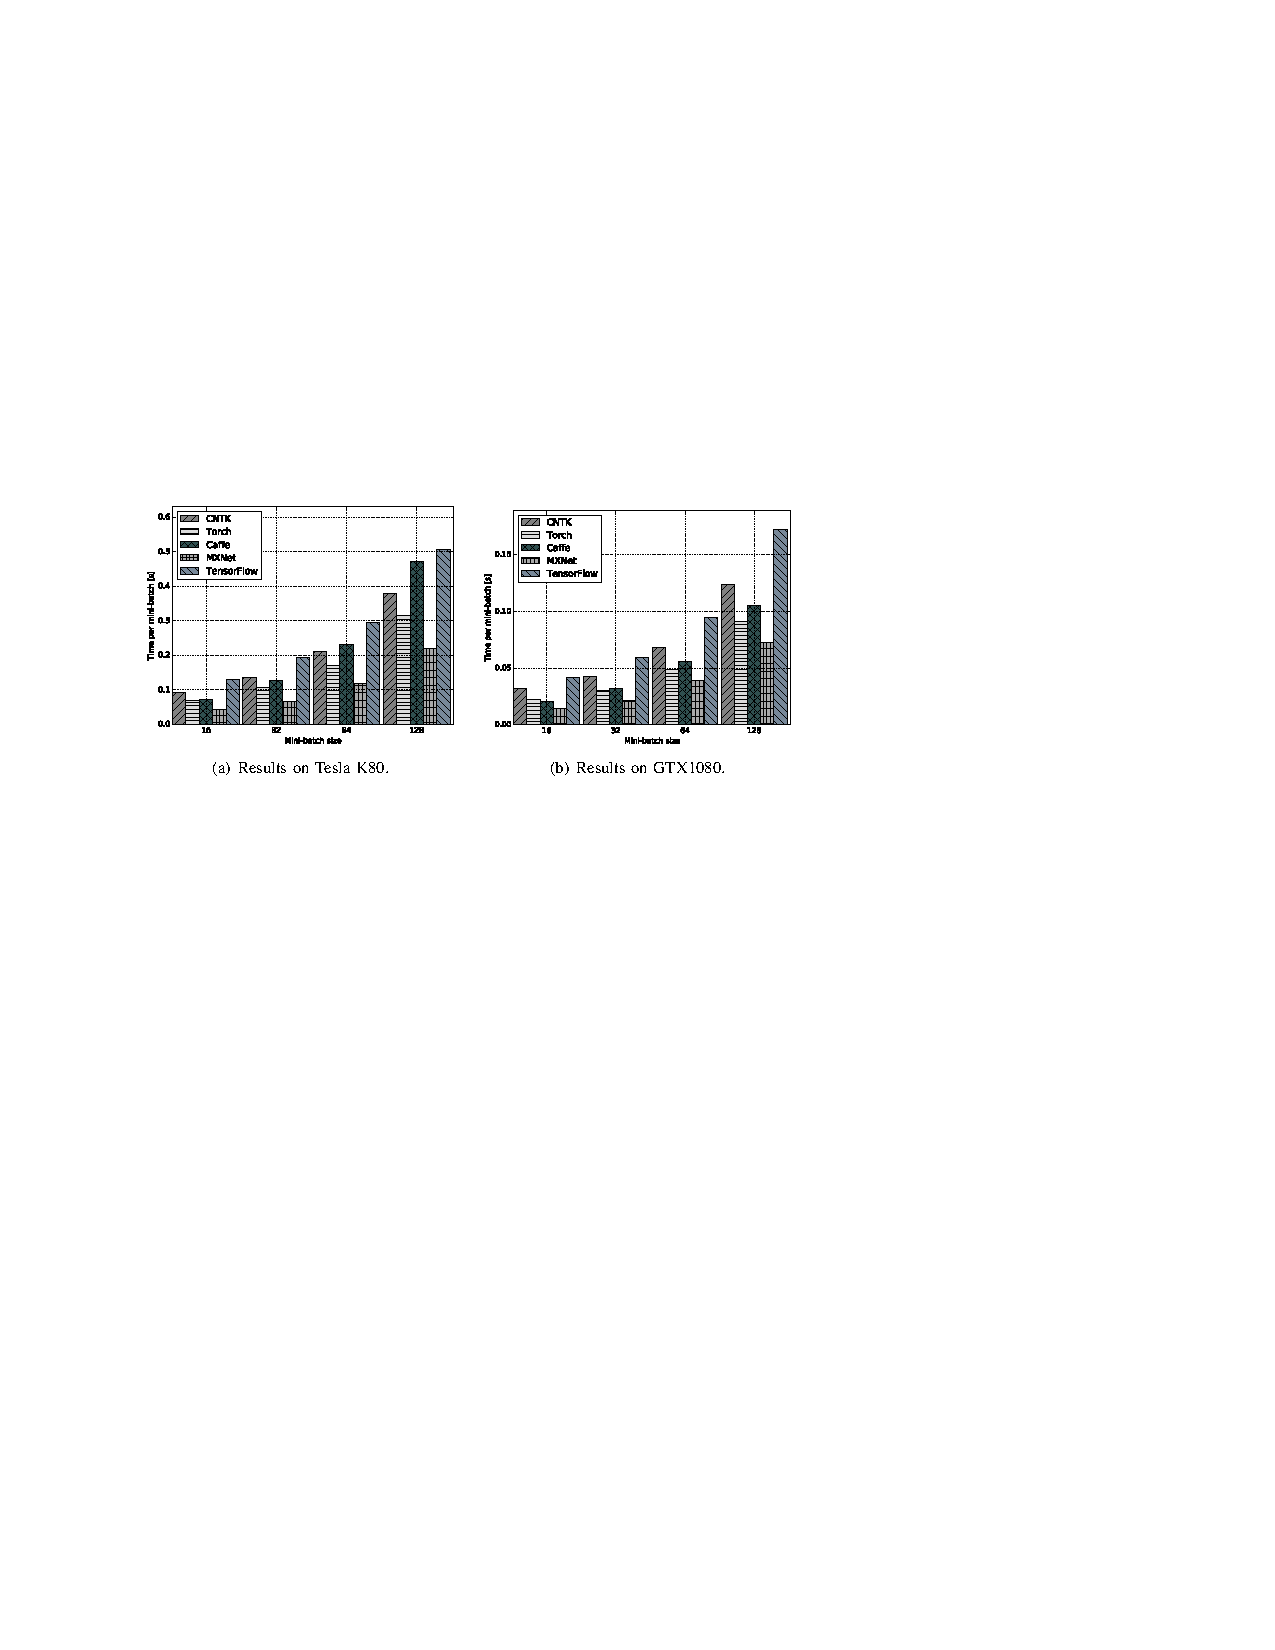
\includegraphics[width=\linewidth]{figures/AlexNet-S2.pdf} 
		\caption{The performance comparison of AlexNet-S on GPU platforms}
	\end{figure}

\vskip -10pt
\begin{mdframed}[style=mystyle1]
\begin{itemize}
\item MXNet out-perform the others for CNN on GPUs
\end{itemize}
\end{mdframed}

\end{frame}

%%%

\begin{frame}
	\MyLogo
	\frametitle{GPU Scalability: CNN Real}

	\begin{figure}[htbp] 
		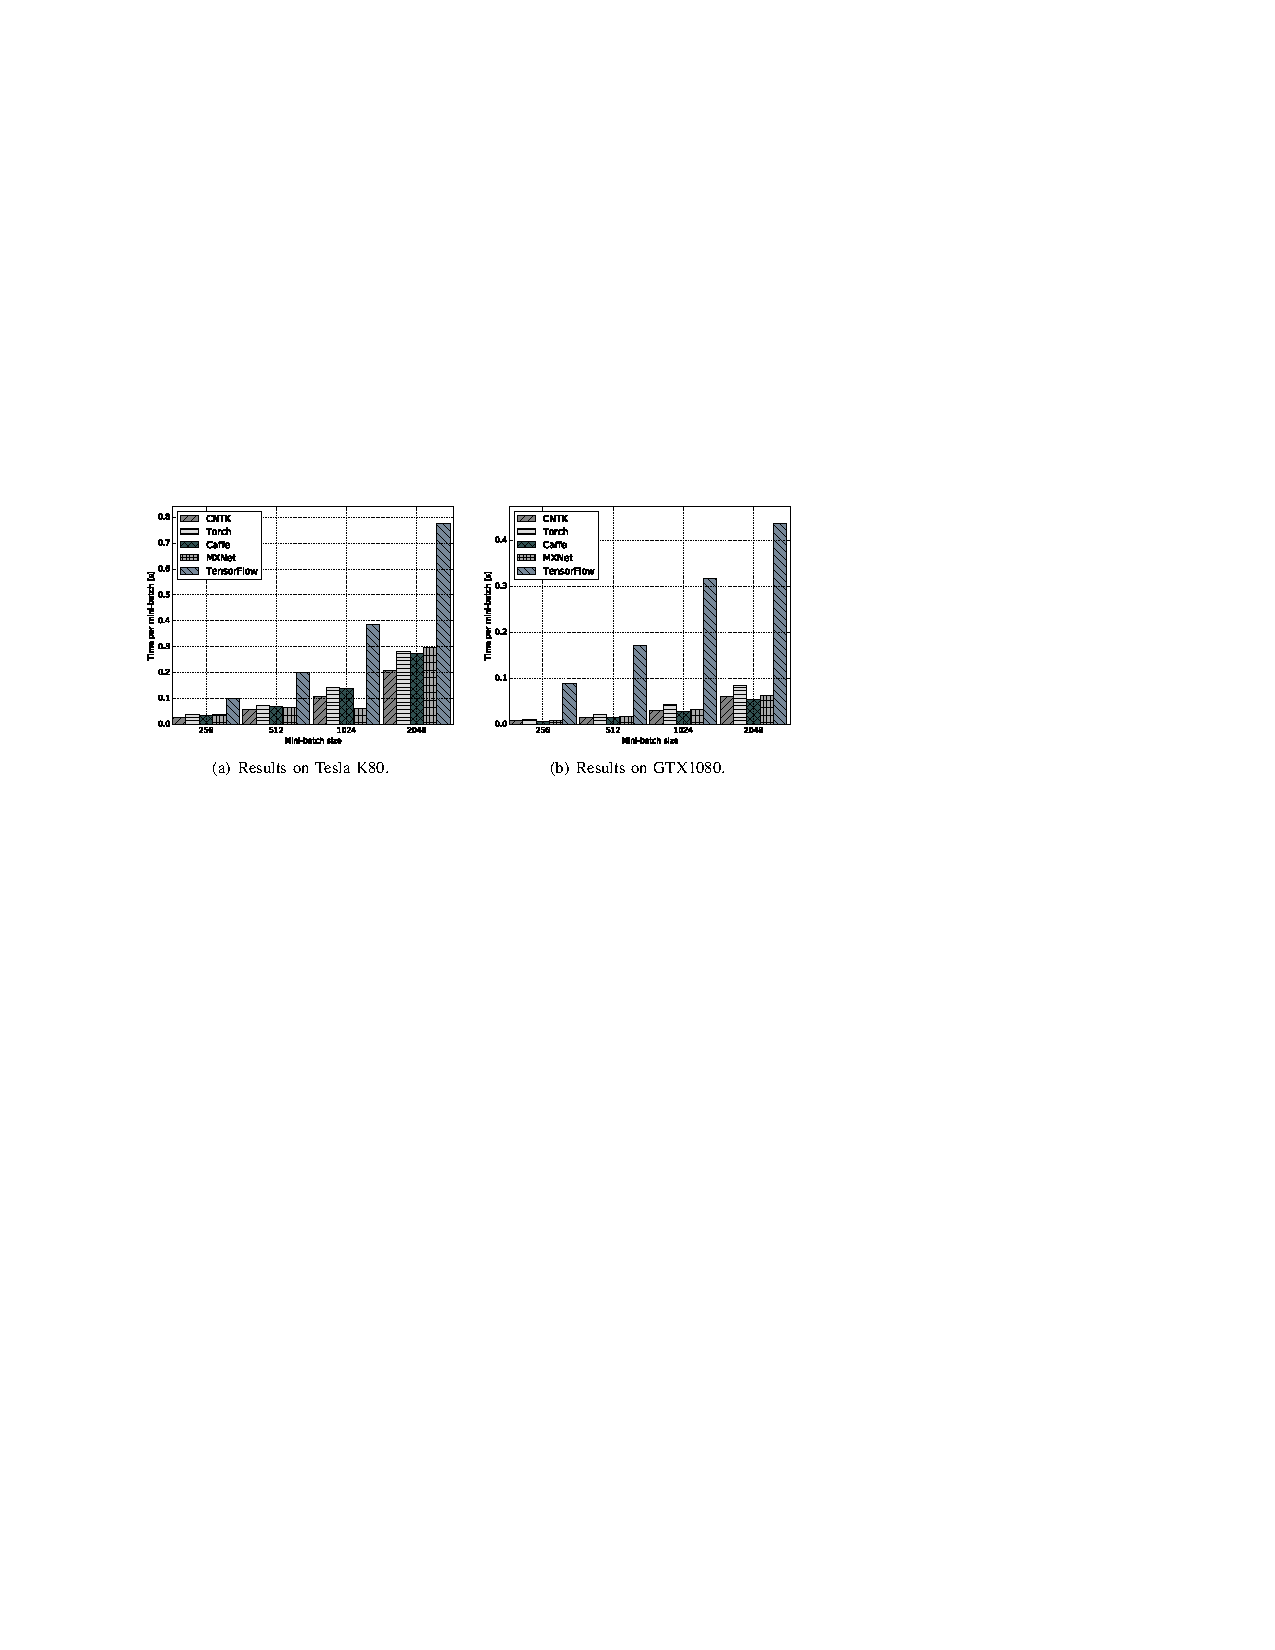
\includegraphics[width=\linewidth]{figures/AlexNet-R2.pdf} 
		\caption{The performance comparison of AlexNet-R on GPU platforms}
	\end{figure}

\vskip -10pt
\begin{mdframed}[style=mystyle1]
\begin{itemize}
\item TensorFlow does not have good GPU performance in general
\end{itemize}
\end{mdframed}

\end{frame}

%%%

\begin{frame}
	\MyLogo
	\frametitle{GPU Scalability: RNN LSTM}
	
	\begin{figure}[htbp] 
		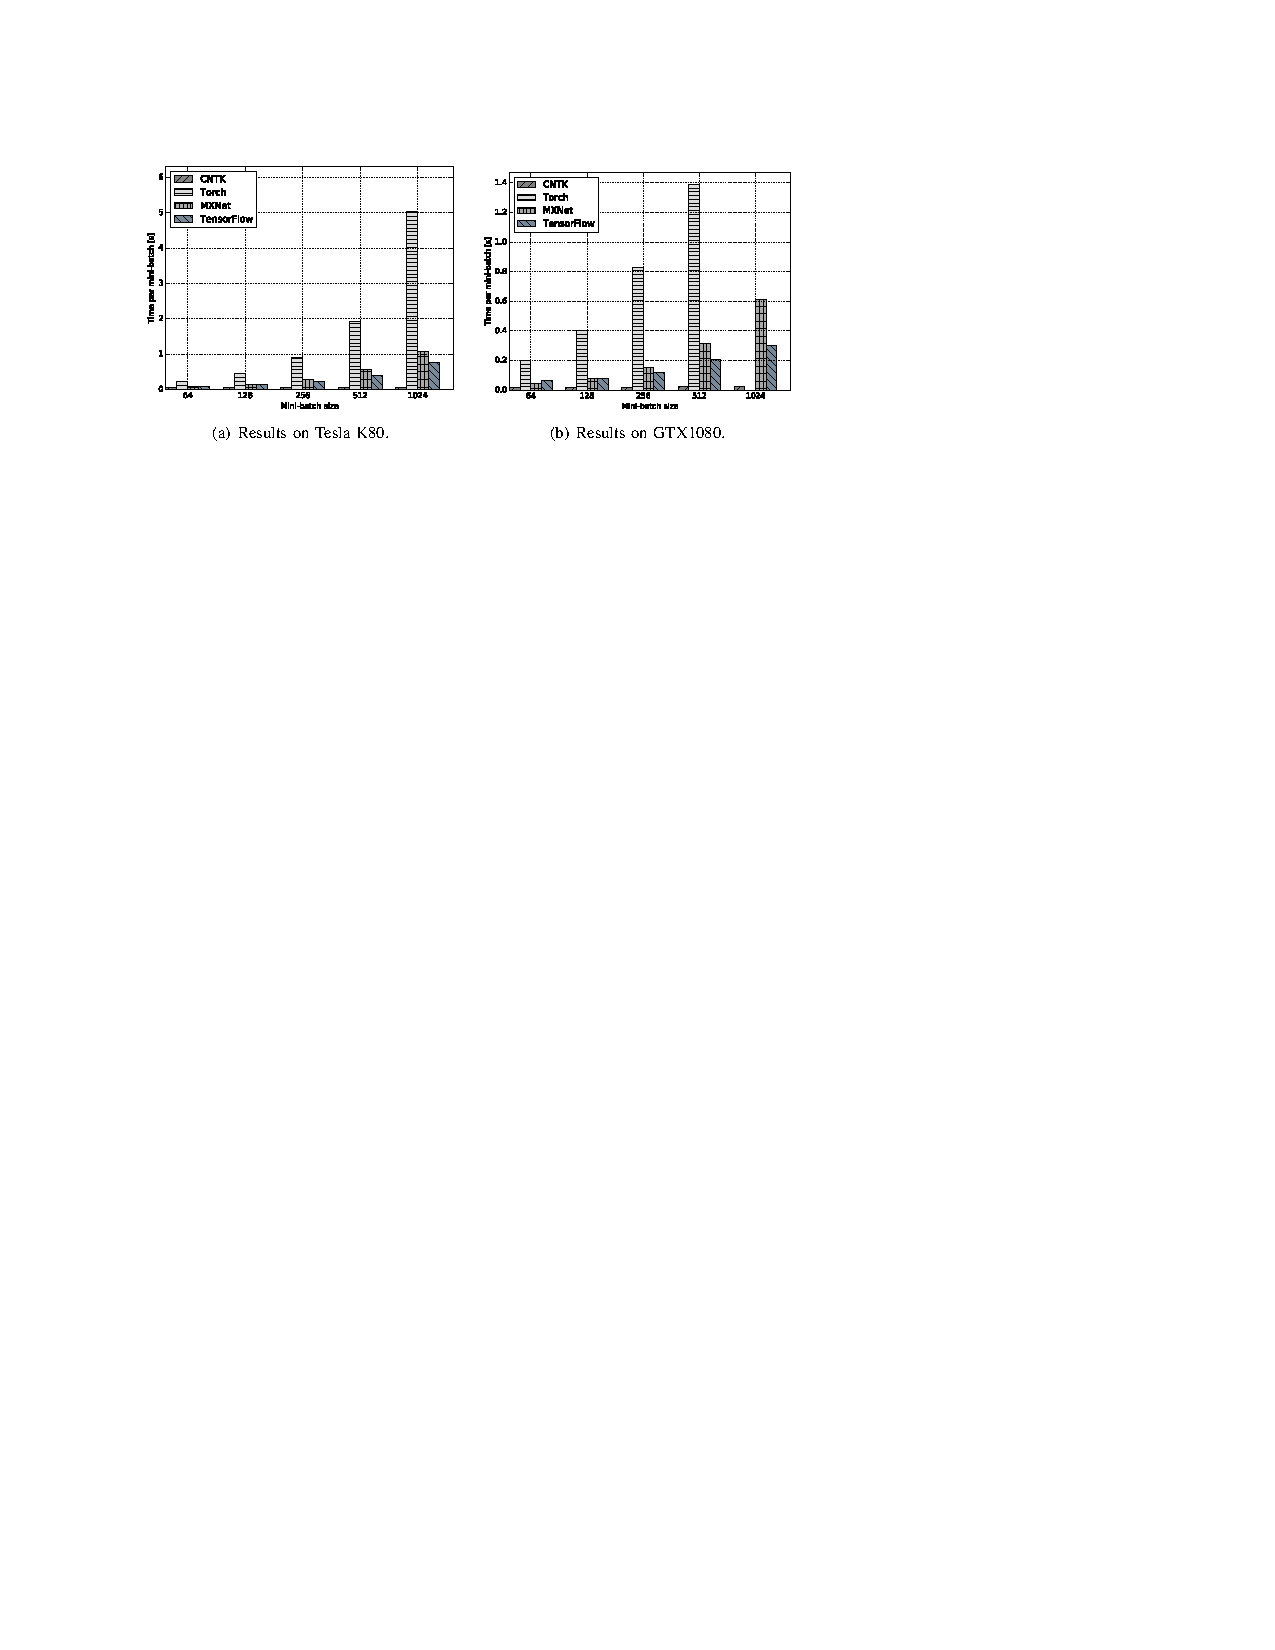
\includegraphics[width=\linewidth]{figures/LSTM2.pdf} 
		\caption{The performance comparison of LSTM on GPU platforms}
	\end{figure}

\vskip -10pt
\begin{mdframed}[style=mystyle1]
\begin{itemize}
\item CNTK has excellent RNN performance both on CPU and GPU
\end{itemize}
\end{mdframed}
	
\end{frame}


\begin{frame}
	\MyLogo
	\frametitle{Multi-GPU Scalability}
	
\begin{figure}[!htbp]%[H]
\centering
\subfloat[Subfigure 1 list of figures text][FCN-R]{
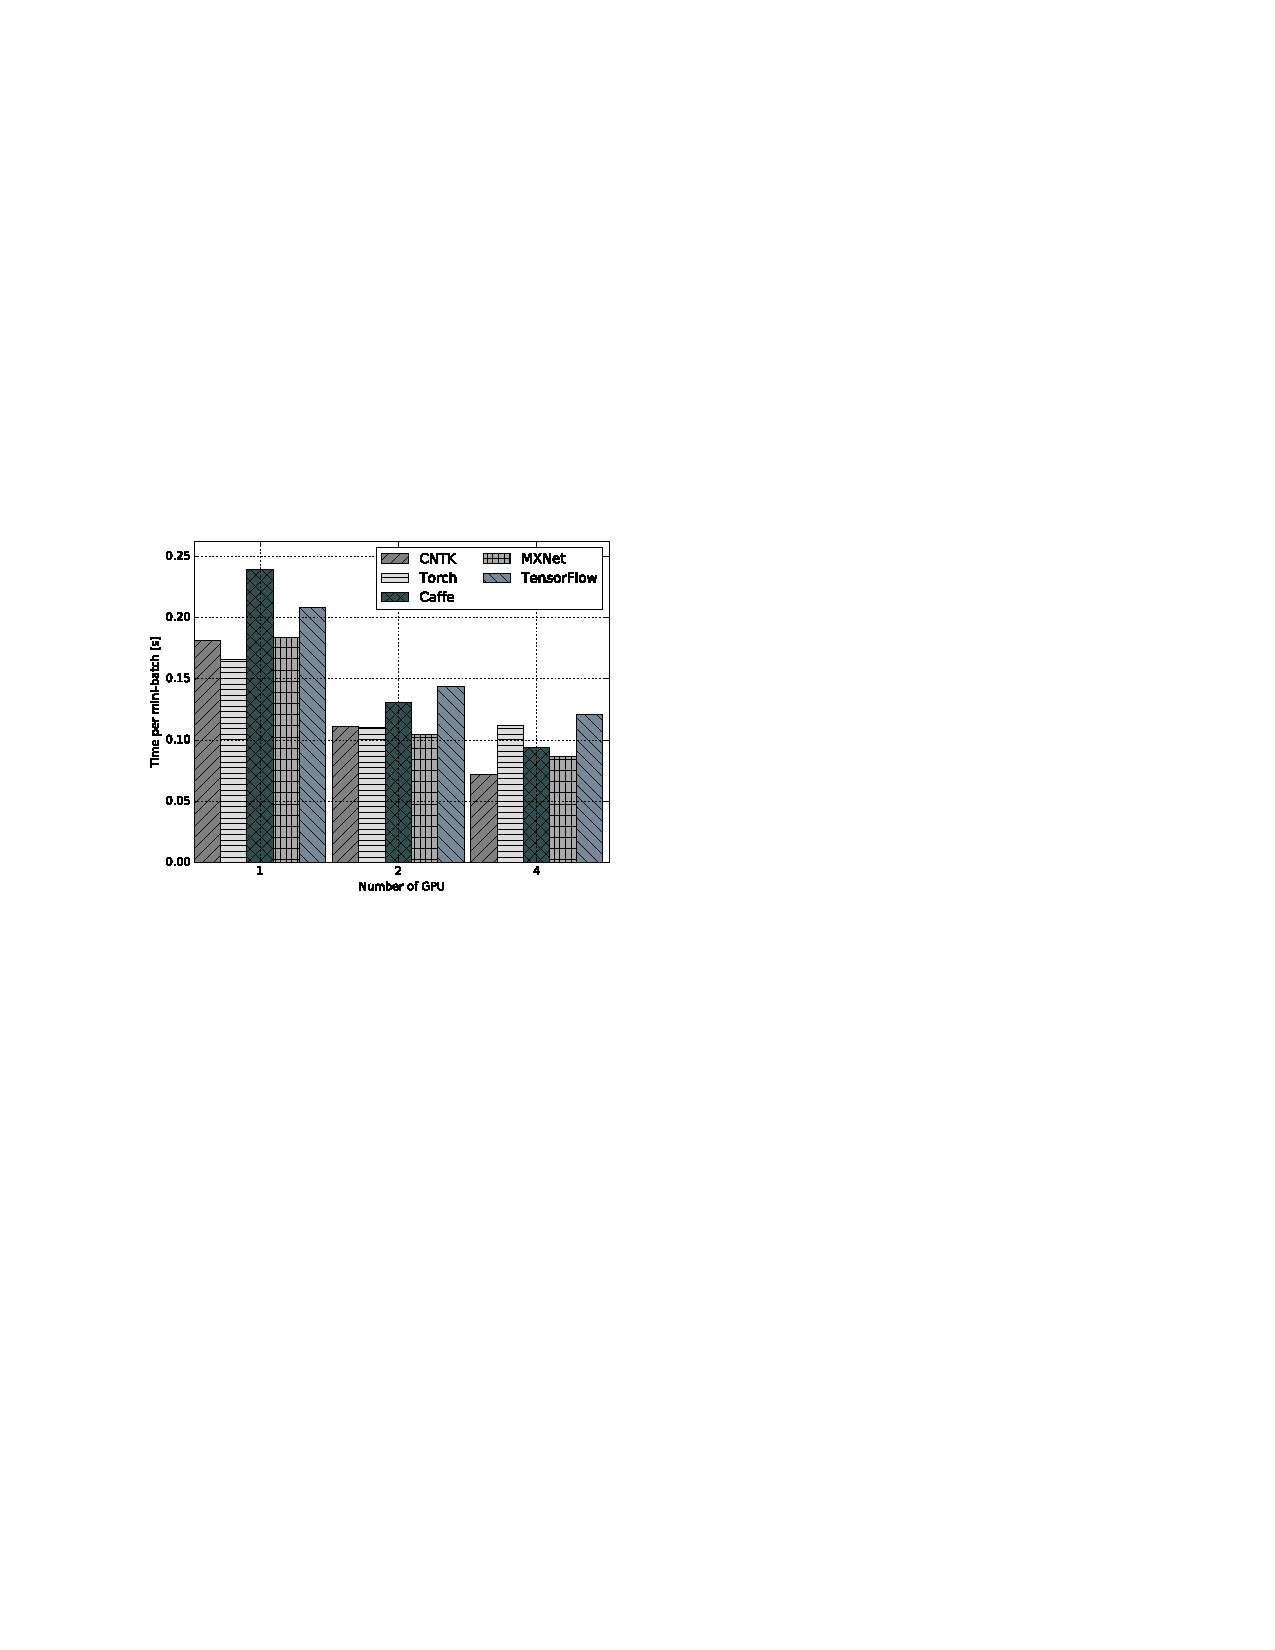
\includegraphics[width=0.33\textwidth]{figures/16a.pdf}
}
\subfloat[Subfigure 2 list of figures text][AlexNet-R]{
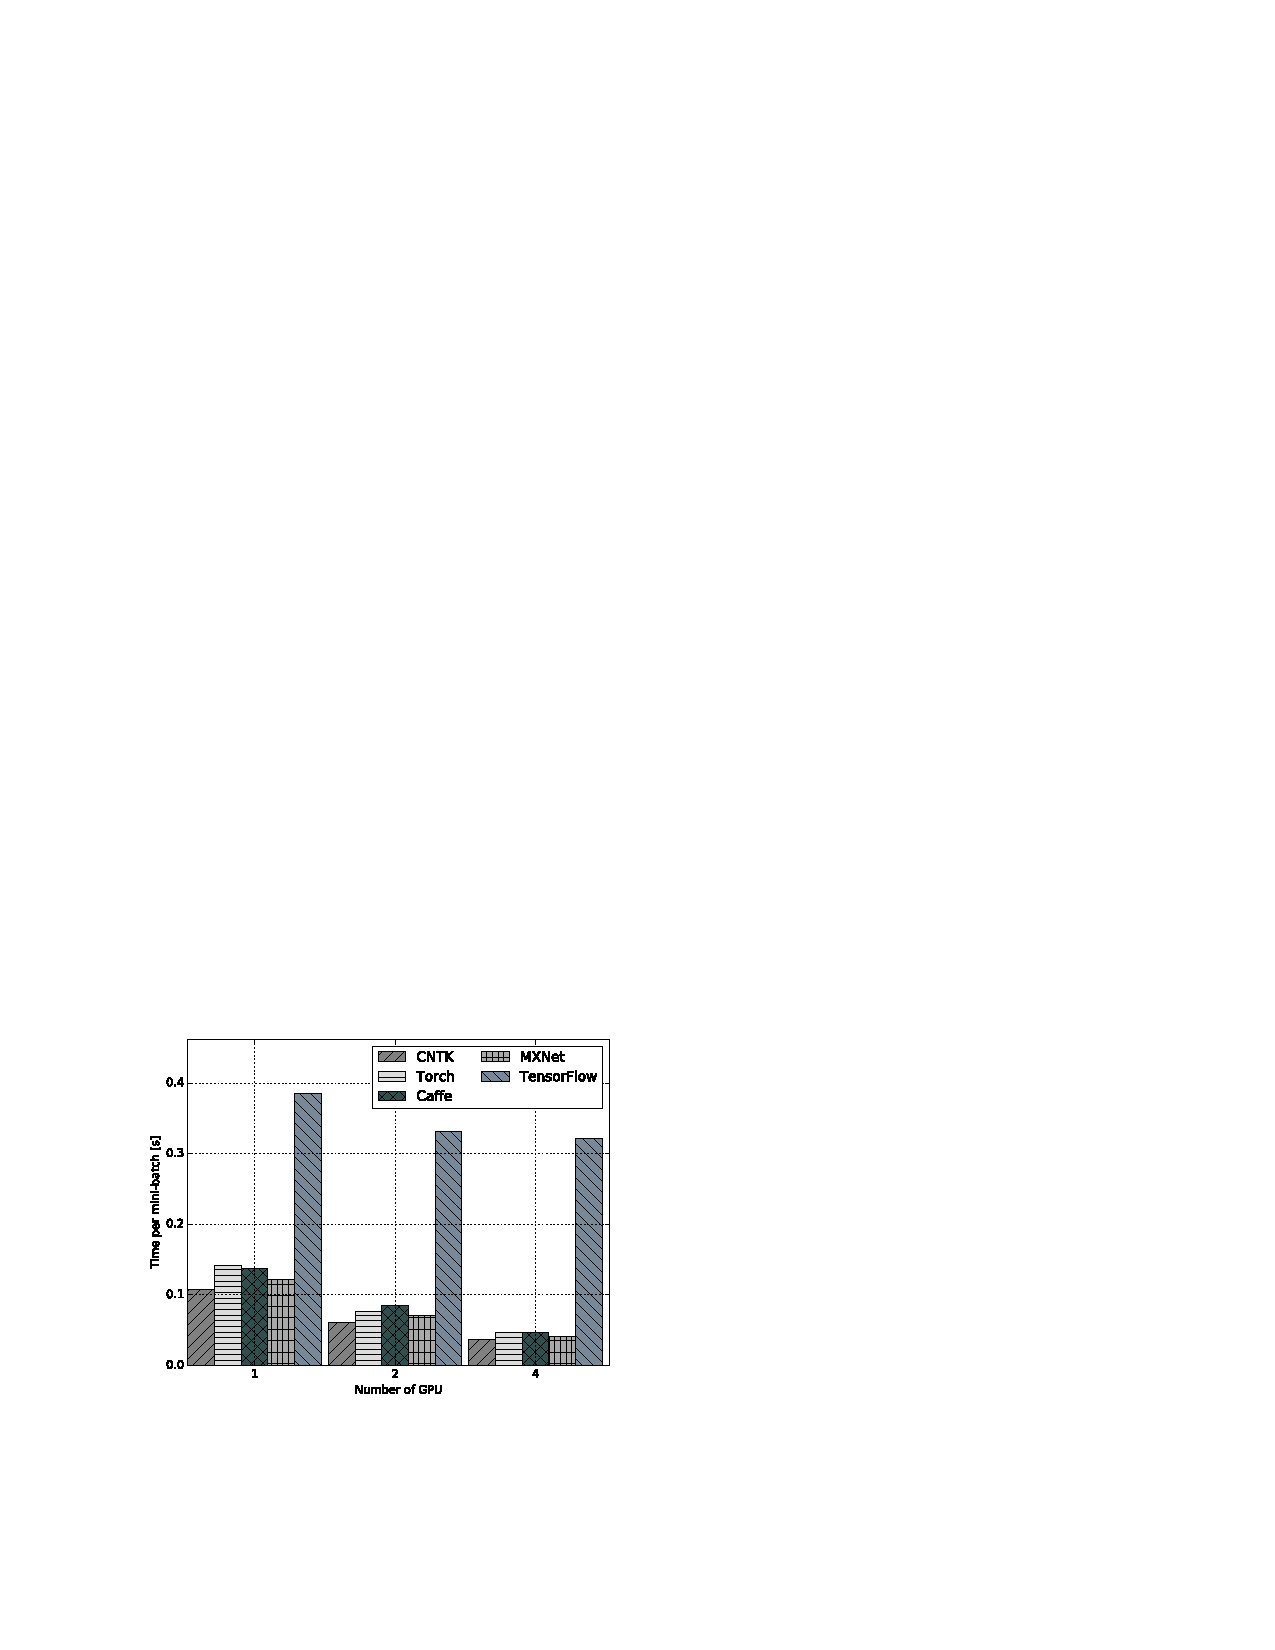
\includegraphics[width=0.33\textwidth]{figures/17a.pdf}
}
\subfloat[Subfigure 2 list of figures text][ResNet-56]{
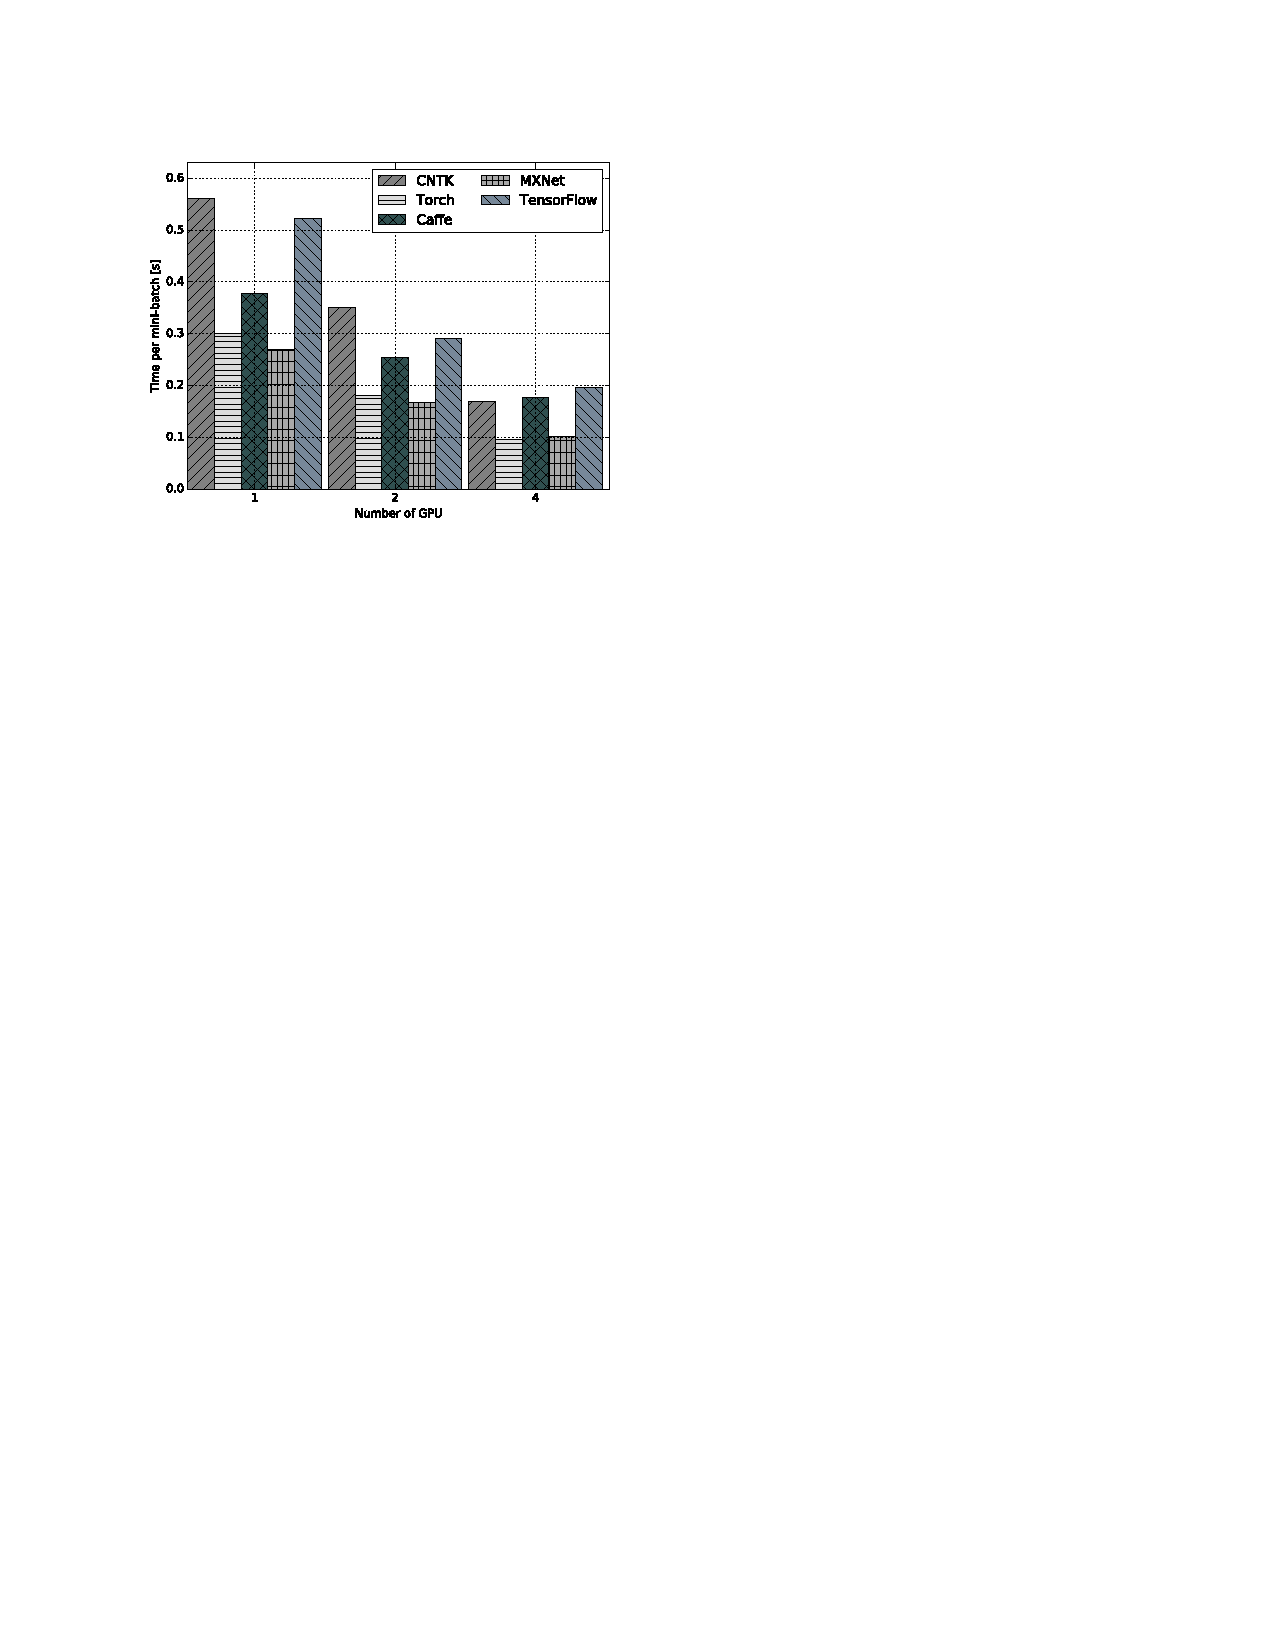
\includegraphics[width=0.33\textwidth]{figures/18a.pdf}
}
\end{figure}

\vskip -10pt
\begin{mdframed}[style=mystyle1]
\begin{itemize}
\item Multi-GPU can greatly boost the training process of network
\item MXNet shows overwhelming advantage over the others
\end{itemize}
\end{mdframed}
\end{frame}

%!TEX root = ../talk.tex

\section{Python}\label{sec:python}

%%%
\subsection{A short introduction on Python}
%%%

\begin{frame}
  \MyLogo
  \frametitle{Python: A general-purpose programming language}  

\small 

\begin{itemize}

\item Created by Guido van Rossum in 1989 and first released in 1991

\item Named after ``the Monty Python'' (British comedy group)

\item An interpreted language---simple, clear, and readable 

\item Python has many excellent packages for machine learning

\item The language of choice in introductory programming courses

\end{itemize}

\begin{figure}[htbp] %  figure placement: here, top, bottom, or page
   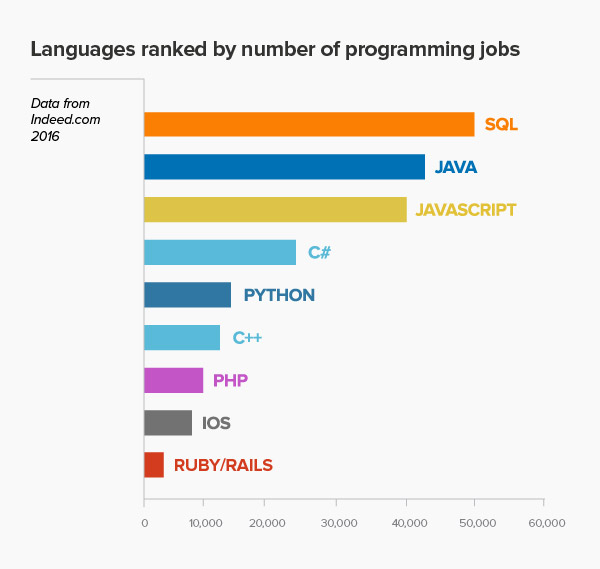
\includegraphics[height=1.7in]{figures/ComputerLanguagesDemand.jpg} 
   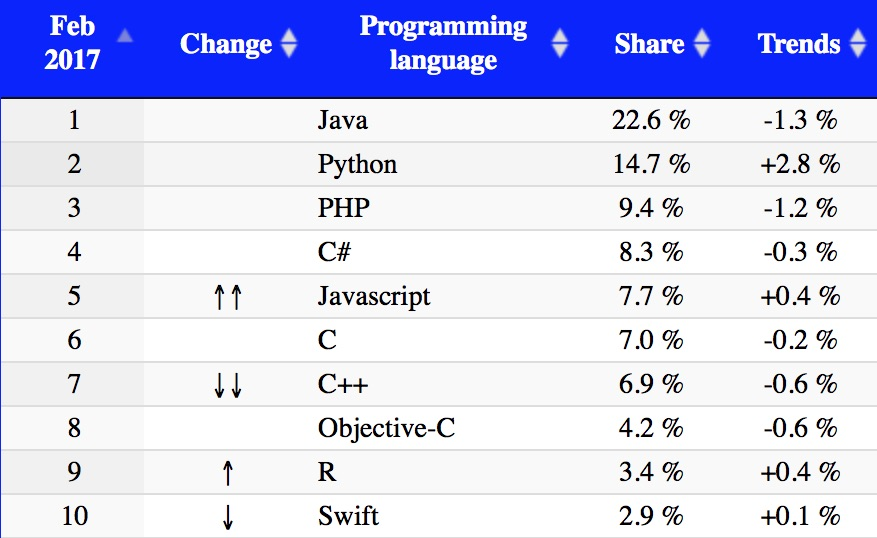
\includegraphics[height=1.7in]{figures/ComputerLanguagesShare.jpg} 
\end{figure}

\end{frame}

%%%

\begin{frame}
  \MyLogo
  \frametitle{Python for Scientific Computing}  

\small

\structure{Why Python for scientific computing?}
\begin{itemize}
	\item Strong introspection\footnote{Code introspection is the ability to examine classes, functions and keywords to know what they are, what they do and what they know.Python provides several functions and utilities for code introspection, like dir(), help(), type().} capabilities (???What does even mean???)
	
	\item Full modularity, supporting hierarchical packages
	\item Exception-based error handling
	\item Dynamic data types and automatic memory management
\end{itemize}

\structure{Why consider such a slow language for simulation?}
\begin{itemize}
	\item Good for proof-of-concept
	\item Implementation time versus execution time
	\item Code readability and maintenance --- short code, fewer bugs
	\item Well-written Python code is ``fast enough'' for most computational tasks
	\item Time critical parts executed through compiled language or \alert{available packages}
\end{itemize}

\end{frame}

%%%
\subsection{Basic language components}
%%%

\begin{frame}[fragile]
  \MyLogo
  \frametitle{Built-in Data Structures}  
\small

\begin{itemize}
	\item[$\bullet$] Numeric types--int, float, complex
	\begin{lstlisting}[language=python]
	For example:
	a=1 int
	b=1.0 float
	c=1L long int
	d=0xf int(hex format)
	e=010 int(octal format)
	f=1+2j complex
	\end{lstlisting}

	\item[$\bullet$] Sequence types--list, tuple, str, dict
	\begin{lstlisting}[language=python]
	For example:
	g=[3.14, True, 'Yes', [1], (1L,)] + [None]*3, list
	h=(3.14, True, 'Yes', [1], ()), tuple
	i='Hello' + "," + '''world!''', str
	j=\{1: 'int', 'pi': 3.14\}, dict
	\end{lstlisting}
\end{itemize}
\end{frame}

%%%

\begin{frame}[fragile]
  \MyLogo
  \frametitle{Control Flow}  
\small

\begin{itemize}
	\item[$\bullet$] If-then-else
	\begin{lstlisting}[language=python]
		a = 1
		if a > 0:
			print "a is positive"
		elif a=0:
			print "a is zero"
		else:
			print "a is negative"
	\end{lstlisting}			
	\item[$\bullet$] For loop
	\begin{lstlisting}[language=python]
		for i in range(10):
			print i
	\end{lstlisting}	
	\item[$\bullet$] While loop
	\begin{lstlisting}[language=python]
		sum = 0; i = 0
		while i < 10:
			sum += i
			i += 1
	\end{lstlisting}
\end{itemize}

\end{frame}

%%%

\begin{frame}[fragile]
  \MyLogo
  \frametitle{Functions and Modules}  
\small

\begin{itemize}
	\item[$\bullet$] Defining functions 
		\begin{lstlisting}[language=python]
			def square(x):
				return x*x
		\end{lstlisting}		
	\item[$\bullet$] Using modules\\
			There are 3 different ways to use modules. Examples are below.\\
			1. import math\\
				This will only introduce the name math into the name space in which the import command was issued. The names within the math module will not appear in the enclosing namespace: they must be accessed through the name math. For example: math.sin(3.14).\\
			2. from math import *\\
				This does not introduce the name math into the current namespace. It does however introduce all public names of the math module into the current namespace, directly using: sin(3.14)\\
			3. from math import sin\\
				This will only import the sin function from math module and introduce the name sin into the current namespace, but it will not introduce the name math into the current namespace, directly using: sin(3.14)
		
\end{itemize}

\end{frame}

%!TEX root = ../talk.tex

\section{TensorFlow}\label{sec:TF}

%%%
\subsection{Computational graph}
%%%

\begin{frame}[fragile]
  \MyLogo
  \frametitle{Computational graph}  
TensorFlow computations are expressed as stateful dataflow graphs.
\begin{itemize}
\item each node corresponds to an operation (eg tensor, add, sub etc)
\item each edge corresponds to tensor flowing direction
\end{itemize}
%  
\begin{columns}
\column{.57\textwidth}
\begin{lstlisting}[language=python]
import tensorflow as tf

graph = tf.Graph()
with graph.as_default():
	with tf.name_scope('input_var'):
		a = tf.Variable(tf.random_uniform([1], -1.0, 1.0))
		tf.summary.histogram('a', a)
		b = tf.Variable(tf.random_uniform([1], -1.0, 1.0))
		tf.summary.histogram('b', b)
	with tf.name_scope('output_var'):
		c = tf.multiply(a, b)
		tf.summary.histogram('c', c)
	merged = tf.summary.merge_all()
	writer = tf.summary.FileWriter('/home/fan/board', graph)

with tf.Session(graph=graph) as sess:
	tf.global_variables_initializer().run()
	writer.add_summary(merged.eval())

\end{lstlisting}
%
\column{.48\textwidth}
%
\begin{figure}[htbp] 
   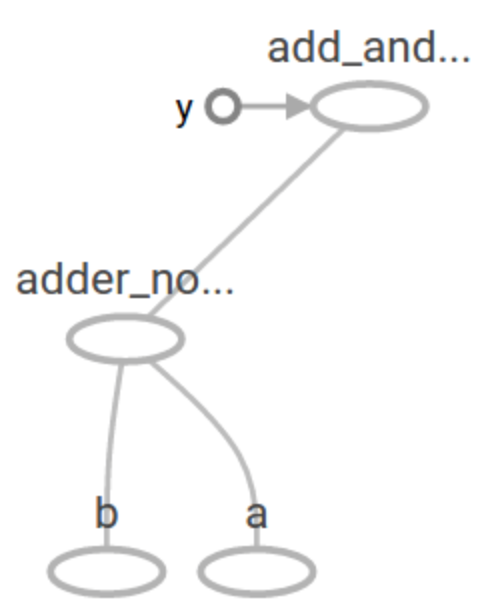
\includegraphics[height=1.5in]{figures/compgraph.png} 
\caption{Computaion graph}
\end{figure}
\end{columns}
\end{frame}

%%%
\subsection{Programming interface}
%%%

\begin{frame}
  \MyLogo
  \frametitle{Programming interface}
  In this section we provide a discussion of the computational graph architecture underlying the TensorFlow software library.
  
  \begin{itemize}
	  	\item Graph: In TensorFlow, machine learning algorithms are represented as computational graph. A computational or dataflow graph is a form of directed graph where vertices or nodes describe operations, while edges represent data flowing between these operations.
	  	
	  	\item Operation: An opreation may represent a mathematical equation, a variable or constant, a control flow directive, a file I/O operation or even a network communication port.
	  	
	  	\item Tensor: A tensor is a multi-dimensional collection of homogeneous values with a fixed, static type.
	  	
	  	\item Variable: Variables can be described as persistent, mutable handles to in-memory buffers storing tensors.
	  	
	  	\item Session: In TensorFlow the execution of operations and evaluation of tensors may only be preformed in a special environment called session.
  \end{itemize}

\end{frame}

%%%
\subsection{Visualization}
%%%

\begin{frame}
  \MyLogo
  \frametitle{Visualization: TensorBoard}  

\begin{columns}
\column{.48\textwidth}  
\scriptsize{
Computation graphs are powerful but complicated
\begin{itemize}
\item  thousands of nodes or more 
\item  network is deep
\item  graph visualization tool TensorBoard is helpful
\end{itemize}
}
%
\column{.5\textwidth}
\begin{figure}[htbp] 
   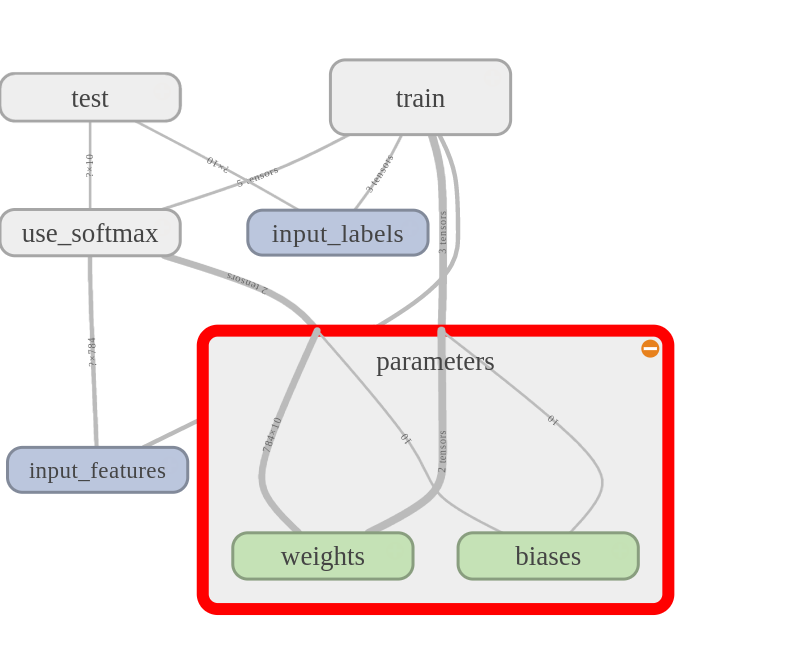
\includegraphics[height=2.5in]{figures/graphvisualization.png} 
\caption{Graph Visualization}
\end{figure}
\end{columns}

\end{frame}

%%%
\subsection{Some examples}
%%%

\begin{frame}[fragile]
  \MyLogo
  \frametitle{Example 1: SoftMax}  
 
\scriptsize{
\begin{lstlisting}[language=python]
import tensorflow as tf

# Import the training data (MNIST)
import tf.examples.tutorials.mnist.input_data as input_data

# Possibly download and extract the MNIST data set
# Retrieve the labels as one-hot-encoded vectors
mnist = input_data.read_data_sets("MNIST_data/", one_hot=True)

# Create a new graph
graph = tf.Graph()

# Set our graph as the one to add nodes to
with graph.as_default():
	# Placeholder for input variables (None = variable dimension)
	x = tf.placeholder("float", shape=[None, 784])
	# Placeholder for labels
	y_ = tf.placeholder("float", shape=[None, 10])
	
	# Weights and bias
	W = tf.Variable(tf.zeros([784, 10]))
	b = tf.Variable(tf.zeros([10])) 
\end{lstlisting}
}
\end{frame}

\begin{frame}[fragile]
  \MyLogo
  \frametitle{Example 1:SoftMax}  
\scriptsize{
\begin{lstlisting}[language=python]
	# Apply softmax regression model
	y = tf.nn.softmax(tf.matmul(x, W) + b)
	
	# Compute the cross entropy of y_ and y
	entropy = -tf.reduce_sum(y_*tf.log(y))
	# Create a gradient-descent optimizer
	train_step = 
		tf.train.GradientDescentOptimizer(0.01).minimize(entropy)
		
	# Find the indices where the predictions were correct
	correct_prediction = tf.equal(tf.argmax(y,1), tf.argmax(y_,1))
	accuracy = tf.reduce_mean(tf.cast(correct_prediction, "float"))

with tf.Session(graph=graph) as session:
	# Initialize all variables
	tf.global_variables_initializer().run()
	
	# Train the model
	for step in range(1000):
		batch_x, batch_y = mnist.train.next_batch(100)
		train_step.run(feed_dict={x: batch_x, y_: batch_y})
	# Print the accuracy using the model
	print accuracy.run(feed_dict={x: mnist.test.images, 
								y_:mnist.test.labels})
\end{lstlisting}
}

%\end{tabular}

%\end{center}
%\label{default}
%\end{table}%
\end{frame}
%!TEX root = ../talk.tex

\section{MXNet}\label{sec:MxNet}

%%%

\frameinlbffalse

{
\usebackgroundtemplate{
\tikz[overlay,remember picture] \node[opacity=0.8, xshift=-3.5cm, at=(current page.east)] {

\includegraphics[width=0.35\paperwidth]{figures/mxnet_logo.jpg}
};}

\begin{frame}[plain]
\frametitle{\S\ref{sec:MxNet}. \insertsection}
\listofframes
\end{frame}
\addtocounter{framenumber}{-1} % this page does not count

}

\frameinlbftrue

%%%
\subsection{Programming interface}
%%%

\begin{frame}
  \MyLogo
  \frametitle{Programming interface}  

\begin{enumerate}
\item Support many scope applications (e.g. computer vision, natural language processing,  speech recognition , unsupervised machine learning, support embedded APIs, visualization)
\item Support many different front-end, including JavaScript (so it be run on web browsers as well)
\item mxnet.ndarray 
\begin{itemize}
\item Similar to numpy.ndarray
\item Supports both CPU and GPU
\end{itemize}

\item Support building neural network graphs
\begin{itemize}
\item Call mx.viz.plot\_network( )
\end{itemize}

\item Mixed programing
\begin{itemize}
\item Suport both imperative and declarative programming 
\end{itemize}
\item Provide intermediate-level and high-level interface modules

\item Provide data parallelism with multi-devices 
%
\item Provide abundant IO functions 
%
\end{enumerate}

\end{frame}

%%%
\subsection{Simple examples}
%%%

\begin{frame}[fragile]
  \MyLogo
  \frametitle{Example: SoftMax in MXNet}  

\begin{lstlisting}[language=python]
import mxnet
import mxnet.symbol as sym
import numpy as np
import numpy.random as random
import time
from minpy.core import function
from minpy.core import grad_and_loss

# define softmax symbol
x_shape = (num_samples, num_classes)
label_shape = (num_samplesm,)
softmax_symbol = sym.SoftmaxOutput(data=sym.Variable('x'), 
                                   name='softmax', grad_scale=1.0/num_samples)

# convert MXNet symbol into a callable function 
# corresponding gradient function
softmax = function(softmax_symbol, [('x', x_shape), ('softmax_label', label_shape)])

# make softmax_label; 
# MXNet's softmax operator does not use one-of-many label format
softmax_label = np.argmax(label, axis=1)

# Redefine loss function using softmax as one operator
def train_loss(w, x):
    y = np.dot(x, w)
    prob = softmax(x=y, softmax_label=softmax_label)
    loss = -np.sum(label * np.log(prob)) / num_samples
    return loss
\end{lstlisting}

\end{frame}

\begin{frame}[fragile]
  \MyLogo
  \frametitle{Example: SoftMax in MXNet (Cont)}  

\ContinueLineNumber
\scriptsize{
\begin{lstlisting}[language=python]
# Initialize weight matrix (again)
weight = random.randn(num_features, num_classes)

# Calculate gradient function automatically
grad_function = grad_and_loss(train_loss)

# Now training it for 100 iterations
start_time = time.time()
for i in range(100):
    dw, loss = grad_function(weight, data)
    if i % 10 == 0:
        print 'Iter {}, training loss {}'.format(i, loss)
    weight -= 0.1 * dw
    
print 'Training time: {}s'.format(time.time() - start_time)
\end{lstlisting}
}

\vskip 100pt

\end{frame}
%!TEX root = ../talk.tex

\section{Torch}\label{sec:Torch}

%%%

\frameinlbffalse

\begin{frame}[plain]
\frametitle{\S\ref{sec:Torch}. \insertsection}
\listofframes
\end{frame}
\addtocounter{framenumber}{-1} % this page does not count

\frameinlbftrue

%%%
\subsection{Programming interface}
%%%

\begin{frame}
  \MyLogo
  \frametitle{Programming interface}  
\begin{enumerate}
\item Wide range of applications
\begin{itemize}
\item Speech, image and video applications
\item  Large-scale machine-learning applications
\end{itemize}
\item Fastest scripting language Lua is used
\item Easily ported to any platform
\begin{itemize}
\item Torch can run on iPhone with no modification to scripts
\end{itemize}
\item Easy extensibility
\begin{itemize}
\item Easy to integrate any library into Torch
\end{itemize}
\end{enumerate}
\end{frame}

%%%
\subsection{Some examples}
%%%

\begin{frame}[fragile]
\MyLogo
\frametitle{Example: Linear Regression}  
\scriptsize{
\begin{lstlisting}[language=python]
require 'torch'
require 'optim'
require 'nn'

# write the loss to a text file and read from there to plot it as training proceeds
logger = optim.Logger('loss_log.txt')

# input data 
data = torch.Tensor{{40,  6,  4},{44, 10,  4},{46, 12,  5},
{48, 14,  7},{52, 16,  9},{58, 18, 12},{60, 22, 14},
{68, 24, 20},{74, 26, 21},{80, 32, 24}}

# define the container
model = nn.Sequential()                 
ninputs = 2; noutputs = 1

# define the only module
model:add(nn.Linear(ninputs, noutputs)) 

# Define a loss function
criterion = nn.MSECriterion()

# retrieve its trainable parameters
x, dl_dx = model:getParameters()

# compute loss function and its gradient 
feval = function(x_new)
   # set x to x_new, if differnt
   if x ~= x_new then
      x:copy(x_new)
   end
\end{lstlisting}
}
\end{frame}

\begin{frame}[fragile]
\MyLogo
\frametitle{Example: Linear Regression}  
\ContinueLineNumber
\scriptsize{
\begin{lstlisting}[language=python]
   # select a new training sample
   _nidx_ = (_nidx_ or 0) + 1
   if _nidx_ > (#data)[1] then _nidx_ = 1 end

   local sample = data[_nidx_]
   local target = sample[{ {1} }]    
   local inputs = sample[{ {2,3} }] 

   # reset gradients
   dl_dx:zero()
 
   # evaluate the loss function and its derivative wrt x
   local loss_x = criterion:forward(model:forward(inputs), target)
   model:backward(inputs, criterion:backward(model.output, target))

   # return loss(x) and dloss/dx
   return loss_x, dl_dx
end

# define SGD 
sgd_params = {
   learningRate = 1e-3,
   learningRateDecay = 1e-4,
   weightDecay = 0,
   momentum = 0
}

# we cycle 10,000 times over our training data
for i = 1,1e4 do
   #this variable is used to estimate the average loss
   current_loss = 0
\end{lstlisting}
}
\end{frame}

\begin{frame}[fragile]
\MyLogo
\frametitle{Example: Linear Regression}  
\ContinueLineNumber
\scriptsize{
\begin{lstlisting}[language=python]
   #an epoch is a full loop over our training data
   for i = 1,(#data)[1] do
      # return new x and value of the loss functions
      _,fs = optim.sgd(feval,x,sgd_params)
      # update loss       
      current_loss = current_loss + fs[1]
   end      
   
   # report average error on epoch
   current_loss = current_loss / (#data)[1]
   print('current loss = ' .. current_loss)
   
   logger:add{['training error'] = current_loss}
   logger:style{['training error'] = '-'}
   logger:plot()  
end

# Test the trained model
text = {40.32, 42.92, 45.33, 48.85, 52.37, 57, 61.82, 69.78, 72.19, 79.42}

for i = 1,(#data)[1] do
   local myPrediction = model:forward(data[i][{{2,3}}])
   print(string.format("%2d %6.2f %6.2f", i, myPrediction[1], text[i]))
end
\end{lstlisting}
}

\vskip 50pt
\end{frame}

\begin{frame}[fragile]
\MyLogo
\frametitle{Example: Two-Layer Network}  
\scriptsize{
\begin{lstlisting}[language=python]
import torch
from torch.autograd import Variable

# N is batch size; D_in is input dimension;
# H is hidden dimension; D_out is output dimension.
N, D_in, H, D_out = 64, 1000, 100, 10

# Create random Tensors to hold inputs and outputs, and wrap them in Variables.
x = Variable(torch.randn(N, D_in))
y = Variable(torch.randn(N, D_out), requires_grad=False)

# Use the nn package to define our model as a sequence of layers.
model = torch.nn.Sequential( torch.nn.Linear(D_in, H),
                             torch.nn.ReLU(),
                             torch.nn.Linear(H, D_out), )

# The nn package also contains definitions of popular loss functions;
loss_fn = torch.nn.MSELoss(size_average=False)

learning_rate = 1e-4

for t in range(500):
	# Forward pass: compute predicted y by passing x to the model.
	y_pred = model(x)
	# Compute and print loss.
	loss = loss_fn(y_pred, y)
	print(t, loss.data[0])
	# Zero the gradients before running the backward pass
	model.zero_grad()
\end{lstlisting}
}
\end{frame}

\begin{frame}[fragile]
\MyLogo
\frametitle{Example: Two-Layer Network}  

\ContinueLineNumber
\begin{lstlisting}[language=python]         
	# Backward pass: compute gradient of the loss
	loss.backward()
         
	# Update the weights using gradient descent
	for param in model.parameters():
		param.data -= learning_rate * param.grad.data
	end
end
\end{lstlisting}

\vskip 125pt

\begin{center}
{\color{red}\scriptsize
https://github.com/jcjohnson/pytorch-examples
}
\end{center}

\end{frame}
%!TEX root = ../talk.tex

\section{Caffe}\label{sec:Caffe}

%%%

\frameinlbffalse

\begin{frame}[plain]
\frametitle{\S\ref{sec:Caffe}. \insertsection}
\listofframes
\end{frame}
\addtocounter{framenumber}{-1} % this page does not count

\frameinlbftrue

%%%
\subsection{Programming interface}
%%%

\begin{frame}
  \MyLogo
  \frametitle{Programming interface}  

\begin{enumerate}
\item Expressive architecture 
\begin{itemize}
\item Define models and optimization by configuration without hard-coding
\item With protocol tool to define parameters for nets and solvers $\ldots$
\end{itemize}
\item Support GPUs 
\item Mainly focus CNN for images
\item Not well documented
\end{enumerate}
\end{frame}

%%%
\subsection{Some examples}
%%%
\begin{frame}[fragile]
  \MyLogo
  \frametitle{Example: Image Classification}  

\begin{lstlisting}[language=python]
import caffe
import matplotlib.pyplot as plt

# paste your image URL here
my_image_url = "https://wikipedia/Orang_Utan/2C_Malaysia.JPG"
!wget -O image.jpg $my_image_url

# transform it and copy it into the net
image = caffe.io.load_image('image.jpg')
caffe.net.blobs['data'].data[...]=transformer.preprocess('data',image)

# perform classification
caffe.net.forward()

# obtain the output probabilities
output_prob = net.blobs['prob'].data[0]

# sort top five predictions from softmax output
top_inds = output_prob.argsort()[::-1][:5]

plt.imshow(image)
print 'probabilities and labels:'
zip(output_prob[top_inds], labels[top_inds])\end{lstlisting}
\end{frame}

%%%

\begin{frame}[fragile]
  \MyLogo
  \frametitle{Example: Extend Layers}  
\begin{lstlisting}[language=python]
import caffe
import numpy as np 

class EuclideanLoss(caffe.layer):
	def setup(self, bottom, top):
		#check input pair
		if len(bottom) != 2:
			raise Exception("Need two inputs to compute distance")
			
	def reshape(self, bottom, top):
		#check input dimensions match
		if bottom[0].count != bottom[1].count:
			raise Exception("Inputs must have the same dimension")
		#difference in shape of inputs
		self.diff = np.zeros_like(bottom[0].data, dtype=np.float32)
		# loss output is scalar
		top[0].reshape(1)
		
	def forward(self, bottom, top):
		self.diff[...] = bottom[0].data - bottom[1].data
		top[0].data[...] = np.sum(self.diff**2)/bottom[0].num/2.	

	def backward(self, top, propagate_down, bottom):
		for i in range(2):
			if not propagate_down[i]:
				continue
			if i == 0:
				sign = 1
			else:
				sign = -1
\end{lstlisting}
\end{frame}

%%%

\begin{frame}[fragile]
  \MyLogo
  \frametitle{Example: Extend Layers}  
  
\ContinueLineNumber
\begin{lstlisting}[language=python]
			bottom[i].diff[...] = sign.self.diff / bottom[1].num
\end{lstlisting}

Define a class in Python to extend Layer
\begin{lstlisting}[language=python]
layer{
	type: "Python"
	python_param {
		module: "laylers"
		layer: "EuclideanLoss"
	}
}
\end{lstlisting}

\tiny
\begin{center}
{
\color{red}https://docs.google.com/presentation/d/1UeKXVgRvvxg9OUdh\_UiC5G71UMscNPlvArsWER41PsU/edit\#slide=id.gc2fcdcce7\_216\_0
}
\end{center}
\end{frame}

%%%

\begin{frame}[plain]
\addtocounter{framenumber}{-1} % this page does not count

\begin{figure}[htbp] %  figure placement: here, top, bottom, or page
   \centering
   
\includegraphics[width=4in]{figures/ThankYou.jpg} 
\end{figure}

\end{frame}

%%%

\end{document}
